% !TeX root = RJwrapper.tex
\title{nortsTest: An R Package for Assessing Normality of Stationary Processes}


\author{by Asael Alonzo Matamoros, Alicia Nieto-Reyes, and Claudio Agostinelli}

\maketitle

\abstract{%
Normality is the central assumption for analyzing dependent data in several time series models, and the literature has widely studied normality tests. However, the implementations of these tests are limited. The nortsTest package is dedicated to fill this void. The package performs the asymptotic and bootstrap versions of the tests of Epps and Lobato and Velasco and the tests of Psaradakis and Vavra, random projections and El Bouch for normality of stationary processes. These tests are for univariate stationary processes but for El Bouch that also allows bivariate stationary processes. In addition, the package offers visual diagnostics for checking stationarity and normality assumptions for the most used time series models in several R packages. This work aims to show the package's functionality, presenting each test performance with simulated examples and the package utility for model diagnostic in time series analysis.
}

\hypertarget{introduction}{%
\section{Introduction}\label{introduction}}

Normality (\emph{a set of observations sampled from a Gaussian process}) is an essential assumption in various statistical models. Therefore, developing procedures for testing this assumption is a topic that has gained popularity over several years. Most existing literature and implementation is dedicated to independent and identically distributed random variables (D'Agostino and Stephens 1986); no results show that these tests are consistent when applied to stationary processes. For this context, several tests have been proposed over the years, but as far as we know, no \texttt{R} package or consistent implementation exists.

The proposed \CRANpkg{nortsTest} package provides seven test implementations to check normality of stationary processes. This work aims to present a review of these tests and introduce the package functionality. Thus, its novelty lies in being the first package and paper dedicated to the implementation of normality tests for stationary processes. The implemented tests are: (i) the asymptotic \emph{Epps} test, (Epps 1987) and (Nieto-Reyes, Cuesta-Albertos, and Gamboa 2014), based on the characteristic function and (ii) its sieve bootstrap approximation (Psaradakis and Vávra 2020), (iii) the corrected \emph{Skewness-Kurtosis} (SK) test implemented by Lobato and Velasco (2004) as an asymptotic test and (iv) by Psaradakis and Vávra (2020) with a sieve bootstrap approximation, (v) the \emph{random projections test} proposed by Nieto-Reyes, Cuesta-Albertos, and Gamboa (2014), which makes use of the tests in (i) and (iii), (vi) the \emph{Psadarakis and Vávra test} (Psaradakis and Vávra 2017) that uses a bootstrap approximation of the Anderson and Darling (1952) test statistic for stationary linear processes and (vii) a normality test by El Bouch, Michel, and Comon (2022) for multivariate dependent samples. Tests (i) to (vi) are for univariate stationary processes.

Furthermore, we propose the \texttt{check\_residual()} function for checking time-series models' assumptions. This function returns a report for stationarity, seasonality, normality tests and visual diagnostics. \texttt{check\_residual()} supports models from the most used packages for time-series analysis, such as the packages \CRANpkg{forecast} (R. Hyndman and Khandakar 2008) and \CRANpkg{aTSA} (Qiu 2015) and even functions in the base \texttt{R} (Team 2018); for instance, it supports the \texttt{HoltWinters} (stats \texttt{R} package) function for the Holt and Winters method (Holt 2004). In addition, the proposed \CRANpkg{nortsTest} package has already been applied in the literature, see Nieto-Reyes (2021) and Nieto-Reyes (2022).

Section 2 provides the theoretical background, including preliminary concepts and results. Section 3 introduces the normality tests for stationary processes, each subsection introducing a test framework and including examples of the tests functions with simulated data. Section 4 provides numerical experiments with simulated data and a real-world application: Subsection 4.1 reports a simulation study for the implemented normality tests and Subsection 4.2 the package's functionality for model checking in a real data application. The \emph{carbon dioxide} data measured in the Malua Loa Observatory (Stoffer 2020) is analyzed using a state space model from the \CRANpkg{forecast} package, evaluating the model's assumptions using our proposed \texttt{check\_residuals()} function. Section 5 discusses the package functionality and provides our conclusions. Furthermore, we mention our future intended work on the package.

\hypertarget{preliminary-concepts}{%
\section{Preliminary concepts}\label{preliminary-concepts}}

This section provides some theoretical aspects of stochastic processes that are a necessary theoretical framework for the following sections. Shumway and Stoffer (2010) and Tsay (2010) give more details of the following definitions and results below.

For the purpose of this work, \(T\) is a set of real values denoted as time, \(T \subseteq \mathbb{R},\) for instance \(T=\mathbb{N}\) or \(T=\mathbb{Z},\) the naturals or integer numbers respectively. We denote by \(X:=\{X_t\}_{t\in T}\) a \textit{stochastic process} with \(X_t\) a real random variable for each \(t\in T.\) Following this notation, a \textit{time-series} is just a finite collection of ordered observations of \(X\) (Shumway and Stoffer 2010). An important measure for a stochastic process is its mean function \(\mu(t) := E[X_t]\) for each \(t \in T\), where \(E[\cdot]\) denotes the usual expected value of a random variable. A generalization of this measure is the k-th order centered moment function \(\mu_k(t) := E[(X_t -\mu(t))^k]\) for each \(t \in T\) and \(k > 1;\) with the process variance function being the second order centered moment, \(\sigma^2(t) := \mu_2(t)\). Other important measures are the auto-covariance and auto-correlation functions, which measure the linear dependency between two different time points of a given process. For any \(t,s \in T,\) they are, respectively,
\[
\gamma(t,s) := E[(X_t -\mu(t))(X_s - \mu(s))] \mbox{ and } \rho(t,s) := \dfrac{\gamma(t,s)}{\sqrt{\mu_2(t)}\sqrt{\mu_2(s)}}.
\]
Other widely used measure functions for the analysis of processes are the skewness and kurtosis functions, defined as \(s(t) := \mu_3(t)/[\mu_2(t)]^{3/2}\) and \(k(t) := \mu_4(t)/[\mu_2(t)]^2\) for each \(t\in T,\) respectively.

A generally used assumption for stochastic processes is stationarity. It has a key role in forecasting procedures of classic time-series modeling (Tsay 2010) or as a principal assumption in de-noising methods for signal theory (Wasserman 2006).

\hypertarget{definition-1}{%
\paragraph{Definition 1}\label{definition-1}}

A stochastic process \(X\) is said to be \emph{strictly stationary} if, for every collection \(\tau = \{t_1,t_2,\ldots, t_k\} \subset T\) and \(h > 0\), the joint distribution of \(\{X_t\}_{t \in \tau}\) is identical to that of \(\{X_{t+h}\}_{t \in \tau}.\)

The previous definition is strong for applications. A milder version of it, which makes use of the process' first two moments, is weak stationarity.

\hypertarget{definition-2}{%
\paragraph{Definition 2}\label{definition-2}}

A stochastic process \(X\) is said to be \emph{weakly stationary} if its mean function is constant in time, \(\mu(t) = \mu\), its auto-covariance function only depends on the difference between times, \(\gamma(s,t) = \sigma|t-s|\) for a \(\sigma\in \mathbb{R}\), and it has a finite variance function, \(\mu_2(t) = \mu_2 < \infty\).

For the rest of this work, the term \emph{stationary} will be used to specify a weakly stationary process. A direct consequence of the stationarity assumption is that the previous measure functions get simplified. Thus, given a stationary stochastic process \(X,\) its mean function, \(k\)-th order centered moment, for \(k>1,\) and auto-covariance function are respectively,
\[
 \mu = E[X_{t_1}]\mbox{, } \mu_k = E[(X_{t_1} -\mu)^k] \mbox{ and } \gamma(h) = E[(X_{t_1+h}-\mu)(X_{t_1}-\mu)],
\]
which are independent of \(t_1\in T.\)

Given a sample \(x_1, \ldots, x_n,\) \(n\in\mathbb{N},\) of equally spaced observations of \(X,\) their corresponding estimators, sample mean, sample \(k\)-th order centered moment and sample auto-covariance, are respectively
\[
 \widehat{\mu} := n^{-1}\sum_{i=1}^nx_i\mbox{, } \widehat{\mu}_k := n^{-1}\sum_{i=1}^n(x_i - \widehat{\mu})^k \mbox{ and }\widehat{\gamma}(h) := n^{-1}\sum_{i = 1}^{n-h}(x_{i+h} - \widehat{\mu})(x_i - \widehat{\mu}).
\]

A particular case in which stationarity implies strictly stationarity is a Gaussian process.

\hypertarget{definition-3}{%
\paragraph{Definition 3}\label{definition-3}}

A stochastic process \(X\) is said to be a \emph{Gaussian process} if for every finite collection \(\tau = \{t_1,t_2,\ldots, t_k\} \subset T,\) the joint distribution of \(\{X_t\}_{t \in \tau}\) has a multivariate normal distribution.

A series of mean zero uncorrelated random variables with finite constant variance is known as \emph{white noise}. If additionally, it is formed of independent and identically distributed (i.i.d) normal random variables, it is known as \emph{Gaussian white noise}; which is a particular case of stationary Gaussian process. For the rest of the work, \(X_t \sim N(\mu,\sigma^2)\) denotes that the random variable \(X_t\) is normally distributed with mean \(\mu\) and variance \(\sigma^2\) and \(\chi^2(v)\) denotes the Chi square distribution with \(v\) degrees of freedom.

Other classes of stochastic processes can be defined using collections of white noise, for instance, the linear process.

\hypertarget{definition-4}{%
\paragraph{Definition 4}\label{definition-4}}

Let \(X\) be a stochastic process. \(X\) is said to be \emph{linear} if it can be written as
\[
X_t = \mu + \sum_{i\in\mathbb{Z}}\phi_i\epsilon_{t-i},
\]
where \(\{\epsilon_i\}_{i\in\mathbb{Z}}\) is a collection of white noise random variables and \(\{\phi_i\}_{i\in\mathbb{Z}}\) is a set of real values such that \(\sum_{i\in\mathbb{Z}} |\phi_j| < \infty.\)

An important class of processes is the \emph{auto-regressive moving average} (\(ARMA\)). George Edward Pelham Box and Jenkins (1990) introduced it for time series analysis and forecast, becoming very well-known in the 90s and early 21st century.

\hypertarget{definition-5}{%
\paragraph{Definition 5}\label{definition-5}}

For any non-negative integers \(p,q,\) a stochastic process \(X\) is an \(ARMA(p,q)\) process if it is a stationary process and
\begin{equation}
  X_t = \sum_{i=0}^p \phi_iX_{t-i}  +\sum_{i=0}^q \theta_i\epsilon_{t-i}, \label{eq:ARMA}
\end{equation}
where \(\{\phi_i\}_{i=0}^p\) and \(\{\theta_i\}_{i=0}^q\) are sequences of real values with \(\phi_0= 0,\) \(\phi_p\neq 0,\) \(\theta_0=1\) and \(\theta_q\neq 0\) and \(\{\epsilon_{i}\}_{i\in\mathbb{Z}}\) is a collection of white noise random variables.

Particular cases of \(ARMA\) processes are those known as auto-regressive (\(AR(p) := ARMA(p,0)\)) and mean average (\(MA(q) := ARMA(0,q)\)) processes. Additionally, a \emph{random walk} is a non stationary AR(1)
process satisfying \eqref{eq:ARMA} with \(p=1,\) \(\phi_1 = 1\) and \(q=0.\) Several properties of an \(ARMA\) process can be extracted from its structure. For that, the \(AR\) and \(MA\) polynomials are introduced
\[
 AR:\text{ } \phi(z) = 1-\sum_{i=0}^p \phi_i z^i \text{ and } MA:\text{ } \theta(z) = \sum_{i=0}^q \theta_i z^i,
\]
where \(z\) is a complex number and, as before, \(\phi_0 = 0,\) \(\phi_p\neq 0,\) \(\theta_0= 1\) and \(\theta_q\neq 0.\) Conditions for stationarity, order selection and, process behavior are properties studied from these two polynomials.

For modeling volatility in financial data, Bollerslev (1986) proposed the \emph{generalized auto-regressive conditional heteroscedastic} (GARCH) class of processes as a generalization of the \emph{auto-regressive conditional heteroscedastic} (ARCH) processes (Engle 1982).

\hypertarget{definition-6}{%
\paragraph{Definition 6}\label{definition-6}}

For any \(p,q \in \mathbb{N}\), a stochastic process \(X\) is a \(GARCH(p,q)\) process if it satisfies \(X_t = \mu + \sigma_{t}\epsilon_t\) with
\[
\sigma_t^2 = \alpha_0 +\sum_{i=1}^p\alpha_i \epsilon_{t-i}^2 +\sum_{i=1}^q \beta_{i}\sigma^2_{t-i}.
\]
\(\mu\) is the process mean, \(\sigma_0\) is a positive constant value, \(\{\alpha_i\}_{i=1}^p\) and \(\{\beta_i\}_{i=1}^q\) are non-negative sequences of real values and \(\{\epsilon_{t}\}_{t \in T}\) is a collection of i.i.d. random variables.

A more general class of processes are the \emph{state-space models} (\(SSMs\)), which have gained popularity over the years because they do not impose on the process common restrictions such as linearity or stationarity and are flexible in incorporating the process different characteristics (Petris, Petrone, and Campagnoli 2007). They are widely used for smoothing (West and Harrison 2006) and forecasting (R. Hyndman and Khandakar 2008) in time series analysis. The main idea is to model the process dependency with two equations: the \emph{state equation}, which models how parameters change over time, and the \emph{innovation equation}, which models the process in terms of the parameters. Some particular SSMs that analyze the level, trend and seasonal components of the process are known as \emph{error, trend, and seasonal} (ETS) models. There are over 32 different variations of ETS models (R. J. Hyndman et al. 2008). One of them is the \emph{multiplicative error, additive trend-seasonality} \((ETS(M,A,A))\) model.

\hypertarget{definition-7}{%
\paragraph{Definition 7}\label{definition-7}}

A SSM process \(X\) follows an ETS(M,A,A) model, if the process accepts\\
\[
X_t = [L_{t-1} +T_{t-1} + S_{t-1}](1 + \epsilon_t)
\]
as innovation equation and
\begin{eqnarray*}L_t &= &L_{t-1} +T_{t-1} +\alpha (L_{t-1} +T_{t-1} +S_{t-m})\epsilon_t\\
    T_t &= &T_{t-1} + \beta (L_{t-1} +T_{t-1} +S_{t-m})\epsilon_t\\
    S_t &= &S_{t-m} + \gamma (L_{t-1} +T_{t-1} +S_{t-m})\epsilon_t,
\end{eqnarray*}\\
as state equations.
\(\alpha, \beta,\gamma \in [0,1]\), \(m\in\mathbb{N}\) denotes the period of the series and \(\{\epsilon_t\}\) are i.i.d normal random variables. For each \(t\in\mathbb{Z},\) \(L_t\), \(T_t\) and \(S_t\) represent respectively the level, trend and seasonal components.

\hypertarget{normality-tests-for-stationary-processes}{%
\section{Normality tests for stationary processes}\label{normality-tests-for-stationary-processes}}

Extensive literature exists on goodness of fit tests for normality under the assumption of independent and identically distributed random variables, including, among others, Pearson's chi-squared test (Pearson and Henrici 1895), Kolmogorov-Smirnov test (Smirnov 1948), Anderson-Darling test (Anderson and Darling 1952), SK test (Jarque and Bera 1980) and Shapiro-Wilk test, (Shapiro and Wilk 1965) and (J. P. Royston 1982). These procedures have been widely used in many studies and applications, see D'Agostino and Stephens (1986) for further details. There are no results, however, showing that the above tests are consistent in the context of stationary processes, in which case the independence assumption is violated. For instance, Gasser (1975) provides a simulation study where Pearson's chi-squared test has an excessive rejection rate under the null hypothesis for dependent data. For this matter, several tests for stationary processes have been proposed over the years. A selection of which we reference here. Epps (1987) provides a test based on the characteristic function, Hinich (1982) proposes a similar test based on the process' spectral density function (Berg, Paparoditis, and Politis 2010, for further insight). Gasser (1975) gives a correction of the SK test, with several modifications made in Lobato and Velasco (2004), Bai and Ng (2005) and Psaradakis (2017), which are popular in many financial applications. Bontemps and Meddahi (2005) constructs a test based on Stein's characterization of a Gaussian distribution. Using the random projection method (Cuesta-Albertos et al. 2007), Nieto-Reyes, Cuesta-Albertos, and Gamboa (2014) build a test that upgrades the performance of Epps (1987) and Lobato and Velasco (2004) procedures. Furthermore, Psaradakis and Vávra (2017) adapts the Anderson and Darling (1952) statistic for stationary linear processes approximating its sample distribution with a sieve bootstrap procedure.

Despite the existing literature, consistent implementations of goodness of fit test for normality of stationary processes in programming languages such as \texttt{R} or \texttt{Python} are limited. This is not the case for normality of independent data, the \CRANpkg{nortest} package (Gross and Ligges 2015) implements tests such as Lilliefors (Dallal and Wilkinson 1986), Shapiro-Francia (P. Royston 1993), Pearson's chi-squared, Cramer von Misses (Anderson 1962) and Anderson-Darling. For a multivariate counterpart, the \CRANpkg{mvnTest} package (Pya et al. 2016) implements the multivariate Shapiro-Wilk, Anderson-Darling, Cramer von Misses, Royston (J. P. Royston 1992), Doornik and Hansen (Doornik and Hansen 2008), Henze and Zirkler (Henze and Zirkler 1990) and the multivariate Chi square test (Vassilly Voinov and Voinov 2016). For the case of dependent data, we present here the \CRANpkg{nortsTest} package. Type within \texttt{R} \texttt{install.packages("nortsTest",\ dependencies\ =\ TRUE)} to install its latest released version from \texttt{CRAN}. \CRANpkg{nortsTest} performs the tests proposed in Epps (1987), Lobato and Velasco (2004), Psaradakis and Vávra (2020), Nieto-Reyes, Cuesta-Albertos, and Gamboa (2014), Psaradakis and Vávra (2017) and El Bouch, Michel, and Comon (2022).

Additionally, the package offers visualization functions for descriptive time series analysis and several diagnostic methods for checking stationarity and normality assumptions for the most used time series models of several \texttt{R} packages. To elaborate on this, Subsection 3.1 introduces the package functionality and software and Subsection 3.2 provides an overview of tests for checking stationary and seasonality. Finally, Subsections 3.3-3.5 present a general framework of each of the implemented normality tests and their functionality by providing simulated data examples.

\hypertarget{software}{%
\subsection{Software}\label{software}}

The package works as an extension of the \CRANpkg{nortest} package (Gross and Ligges 2015), which performs normality tests in random samples but for independent data. The building block functions of the \CRANpkg{nortsTest} package are:

\begin{itemize}
\item
  \texttt{epps.test()}, function that implements the test of Epps,
\item
  \texttt{epps\_bootstrap.test()}, function that implements a bootstrap approximation of the test of Epps,
\item
  \texttt{lobato.test()}, function that implements the asymptotic test of Lobato and Velasco,
\item
  \texttt{lobato\_bootstrap.test()}, function that implements a bootstrap approximation of the test of Lobato and Velasco,
\item
  \texttt{rp.test()}, function that implements the random projection test of Nieto-Reyes, Cuesta-Albertos and Gamboa,
\item
  \texttt{vavra.test()}, function that implements the test of Psaradaki and Vavra, and
\item
  \texttt{elbouch.test()}, function that implements the test of El Bouch, Michel and Comon.
\end{itemize}

Each of these functions accepts a \texttt{numeric} (\emph{numeric}) or \texttt{ts} (\emph{time series}) class object for storing data, and returns a \texttt{htest} (\emph{hypothesis test}) class object with the main results for the test. To guarantee the accuracy of the results, each test performs unit root tests for checking stationarity and seasonality (see Subsection 3.2) and displays a warning message if any of them is not satisfied.

For visual diagnostic, the package offers different plot functions based on the \CRANpkg{ggplot2} package (Wickham 2009): the \texttt{autoplot()} function plots \texttt{numeric}, \texttt{ts} and \texttt{mts} (\emph{multivariate time series}) classes while the \texttt{gghist()} and \texttt{ggnorm()} functions are for plotting histogram and qq-plots respectively; and on the \CRANpkg{forecast} package (R. Hyndman and Khandakar 2008): \texttt{ggacf()} and \texttt{ggPacf()} for the display of the auto-correlation and partial auto-correlations functions respectively.

Furthermore, inspired in the function \texttt{checkresiduals()} of the \CRANpkg{forecast} package, we provide the \texttt{check\_residuals()} function to test the model assumptions using the estimated residuals. The upgrade of our proposal is that, besides providing plots for visual diagnosis (setting the \texttt{plot} option as \texttt{TRUE}), it does check stationarity, seasonality (\emph{Subsection 3.2}) and normality, presenting a report of the used tests and conclusions for assessing the model's assumptions. An illustration of these functions is provided in Subsection 4.2, where we show the details of the functions and their utility for assumptions commonly checked in time series modeling.

\hypertarget{tests-for-stationarity}{%
\subsection{Tests for stationarity}\label{tests-for-stationarity}}

For checking stationarity, the \CRANpkg{nortsTest} package uses \textit{unit root} and \textit{seasonal unit root} tests. These tests work similarly, checking whether a specific process follows a random walk model, which clearly is a non-stationary process.

\hypertarget{unit-root-tests}{%
\subsubsection{Unit root tests}\label{unit-root-tests}}

A linear stochastic process \(X\) that follows a random walk model is non stationary. Its AR polynomial is \(\phi(z) = 1 - z\), whose solution (root) is unique and equal to one. Thus, it is common to test the non stationarity of a linear process by checking whether its AR polynomial has a unit root (a root equal to one).

The most commonly used tests for unit root testing are \emph{Augmented Dickey-Fuller} (Said and Dickey 1984), \emph{Phillips-Perron} (Perron 1988), \emph{kpps} (Kwiatkowski et al. 1992) and \textit{Ljung-Box} (G. E. P. Box and Pierce 1970). In particular, the \emph{Ljung-Box} test contrasts the null auto-correlation hypothesis of identically distributed Gaussian random variables, which is equivalent to test stationarity. The \texttt{uroot.test()} and \texttt{check\_residual()} functions perform these tests, making use of the \CRANpkg{tseries} package (Trapletti and Hornik 2019).

\hypertarget{seasonal-unit-root-tests}{%
\subsubsection{Seasonal unit root tests}\label{seasonal-unit-root-tests}}

Let \(X\) be a stationary process and \(m\) its period. Note that for observed data, \(m\) generally corresponds to the number of observations per unit of time. \(X\) follows a seasonal random walk if it can be written as
\[
 X_t = X_{t-m} + \epsilon_t,
\]
where \(\epsilon_t\) is a collection of i.i.d random variables. In a similar way, the process \(X\) is non-stationary if it follows a seasonal random walk. Or equivalently, \(X\) is non stationary if the seasonal AR(1) polynomial (\(\phi_m(z) = 1 - \phi z^m\)) has a unit root. The \texttt{seasonal.test()} and \texttt{check\_residuals()} functions perform the \emph{OCSB test} (Osborn et al. 1988) from the \CRANpkg{forecast} package and the \emph{HEGY} (Beaulieu and Miron 1993) and \emph{Ch} (Canova and Hansen 1995) tests from the \CRANpkg{uroot} package (López-de-Lacalle 2019).

\hypertarget{tests-of-epps}{%
\subsection{Tests of Epps}\label{tests-of-epps}}

The \(\chi^2\) test for normality proposed by Epps (1987) compares the empirical characteristic function of the one-dimensional marginal of the process with the one of a normally distributed random variable evaluated at certain points on the real line. Several authors, including Lobato and Velasco (2004), Psaradakis and Vávra (2017) and El Bouch, Michel, and Comon (2022), point out that the greatest challenge in the Epps' test is its implementation procedure, which we address with the \CRANpkg{nortsTest} package. Other existing tests based on the empirical characteristic function of the one-dimensional marginal of the process include Hong (1999) and the references therein. This test differs, however, in that it uses spectral analysis and derivatives.

Furthermore, Meintanis (2016) reviews on testing procedures based on the empirical characteristic function. There, it is commented about the random projection test (Nieto-Reyes, Cuesta-Albertos, and Gamboa 2014, and here below) as a recent development of Epps' test. In fact, in Nieto-Reyes, Cuesta-Albertos, and Gamboa (2014) the consistency of Epps test is improved by taking at random the elements at which the characteristic function is evaluated. Additionally, El Bouch, Michel, and Comon (2022) proposes a sieve bootstrap modification of the Epps' test. In addition to the classical asymptotic Epps' test, we include these last two approaches here, and in the package, see the Example below and the paragraph before it. Let us provide now the foundation behind the Epps' tests.

Let \(X\) be a stationary stochastic process that satisfies
\begin{equation}
  \sum_{t=-\infty}^{\infty}|t|^k|\gamma(t)| <\infty \mbox{ for some } k >0. \label{eq:a}
\end{equation}
The null hypothesis is that the one-dimensional marginal distribution of \(X\) is a Gaussian process. The procedure for constructing the test consists of defining a function \(g\), estimating its inverse spectral matrix function, minimizing the generated quadratic function in terms of the unknown parameters of the random variable and, finally, obtaining the test statistic, which converges in distribution to a \(\chi^2.\)

Given \(N \in\mathbb{N}\) with \(N \geq 2,\) let
\[
\Lambda :=\{\lambda:=(\lambda_1, \ldots, \lambda_N) \in \mathbb{R}^N: \lambda_i \leq \lambda_{i+1} \text{ and } \lambda_i > 0, \text{ for }  i = 1,2,\ldots, N \},
\]
and \(g:\mathbb{R}\times \Lambda \rightarrow \mathbb{R}^n\) be a measurable function, where
\[
 g(x,\lambda):= [\cos(\lambda_1x),\sin(\lambda_1x),\ldots,\cos(\lambda_Nx),\sin(\lambda_Nx)].
\]
Additionally, let \(g_\theta:\Lambda \rightarrow \mathbb{R}^N\) be a function defined by
\[
 g_\theta(\lambda) := \left[\mbox{Re}(\Phi_\theta(\lambda_1)),\mbox{Im}(\Phi_\theta(\lambda_1)),\ldots,\mbox{Re}(\Phi_\theta(\lambda_N)),\mbox{Im}(\Phi_\theta(\lambda_N))  \right]^t,
\]
where the \(\mbox{Re}(\cdot)\) and \(\mbox{Im}(\cdot)\) are the real and imaginary components of a complex number and \(\Phi_\theta\) is the characteristic function of a normal random variable with parameters \(\theta := (\mu,\sigma^2)\in \Theta,\) an open bounded set contained in \(\mathbb{R}\times \mathbb{R}^+\). For any \(\lambda\in\Lambda,\) let us also denote
\[
 \widehat{g}(\lambda) := \dfrac{1}{n}\sum_{t=1}^n [\cos(\lambda_1 x_t),\sin(\lambda_1x_t),\ldots,\cos(\lambda_N x_t),\sin(\lambda_N x_t)]^t.
\]
Let \(f(v;\theta,\lambda)\) be the spectral density matrix of \(\{g(X_t,\lambda)\}_{t \in\mathbb{Z}}\) at a frequency \(v.\)
Then, for \(v = 0\), it can be estimated by
\[
 \widehat{f}(0;\theta,\lambda) := \dfrac{1}{2\pi n}\left(\sum_{t=1}^n  \widehat{G}(x_{t,0},\lambda) +2\sum_{i=1}^{\lfloor  n^{2/5}\rfloor}(1 -i/\lfloor n^{2/5}  \rfloor)\sum_{t=1}^{n-i}\widehat{G}(x_{t,i},\lambda) \right),
\]
where \(\widehat{G}(x_{t,i},\lambda) = (\widehat{g}(\lambda) -g(x_{t},\lambda))(\widehat{g}(\lambda) -g(x_{t+i},\lambda))^t\) and \(\lfloor \cdot \rfloor\) denotes the floor function. The test statistic general form under \(H_0\) is
\[
 Q_n(\lambda) := \min_{\theta \in \Theta} \left\{ Q_n(\theta,\lambda) \right\},
\]
with
\[
 Q_n(\theta,\lambda):=(\widehat{g}(\lambda)-g_\theta(\lambda))^tG_n^+(\lambda)(\widehat{g}(\lambda)-g_\theta(\lambda)),
\]
where \(G^{+}_n\) is the generalized inverse of the spectral density matrix \(2 \pi \widehat{f}(0;\theta,\lambda)\). Let
\[
 \widehat{\theta} := \arg \min_{\theta \in \Theta} \left\{ Q_n(\theta,\lambda) \right\},
\]
be the argument that minimizes \(Q_n(\theta,\lambda)\) such that \(\widehat{\theta}\) is in a neighborhood of \(\widehat{\theta}_n := (\widehat{\mu},\widehat{\gamma}(0))\). To guarantee its' existence and uniqueness, the following assumptions are required. We refer to them as assumption \((A.)\).

\((A.)\) Let \(\theta_0\) be the true value of \(\theta\) under \(H_0\), then for every \(\lambda \in \Lambda\) the following conditions are satisfied.

\begin{itemize}
\item
  \(f(0;\theta,\lambda)\) is positive definite.
\item
  \(\Phi_\theta(\lambda)\) is twice differential with respect to \(\theta\) in a neighborhood of \(\theta_0\).
\item
  The matrix \(D(\theta_0,\lambda) = \dfrac{\partial \Phi_\theta(\lambda)}{\partial\theta |_{\theta = \theta_0}} \in \mathbb{R}^{N\times 2}\) has rank 2.
\item
  The set \(\Theta_0(\lambda) := \{ \theta \in \Theta: \Phi_\theta(\lambda_i) = \Phi_{\theta_0}(\lambda_i), i=1, \ldots,N\}\) is a finite bounded set in \(\Theta\). And \(\theta\) is a bounded subset \(\mathbb{R}\times \mathbb{R}^+\).
\item
  \(f(0;\theta,\lambda) = f(0;\theta_0,\lambda)\) and \(D(\theta_0,\lambda) = D(\theta_,\lambda)\) for all \(\theta \in \Theta_0(\lambda)\).
\end{itemize}

Under these assumptions, the Epps's main result is presented as follows.

\hypertarget{theorem-1-epps1987-theorem-2.1}{%
\paragraph{Theorem 1 (Epps 1987, Theorem 2.1)}\label{theorem-1-epps1987-theorem-2.1}}

Let \(X\) be a stationary Gaussian process such that \eqref{eq:a} and \((A.)\) are satisfied, then \(nQ_n(\lambda)\to_d \chi^2(2N - 2)\) for every \(\lambda \in \Lambda\).

The current \CRANpkg{nortsTest} version, uses \(\Lambda := \{\verb|lambda|/\widehat{\gamma}(0)\}\) as the values to evaluate the empirical characteristic function, where \(\widehat{\gamma}(0)\) is the sample variance. By default \texttt{lambda\ =\ c(1,\ 2)}. Therefore, the implemented test statistic converges to a \(\chi^2\) distribution with two degrees of freedom. The user can change these \(\Lambda\) values as desired by simply specifying the function's \texttt{lambda} argument, as we show in the Example below.

\hypertarget{example-1}{%
\paragraph{Example 1}\label{example-1}}

A stationary \(AR(2)\) process is drawn using a beta distribution with \texttt{shape1\ =\ 9} and \texttt{shape2\ =\ 1} parameters, and performed the implementation of the test of Epps, \texttt{epps.test()}. At significance level \(\alpha = 0.05\), the null hypothesis of normality is correctly rejected.

\begin{verbatim}
set.seed(298)
x = arima.sim(250,model = list(ar =c(0.5,0.2)),
                 rand.gen = rbeta,shape1 = 9,shape2 = 1)

# Asymptotic Epps test
epps.test(x)
#> 
#>  Epps test
#> 
#> data:  x
#> epps = 22.576, df = 2, p-value = 1.252e-05
#> alternative hypothesis: x does not follow a Gaussian Process
\end{verbatim}

Asymptotic Epps test with random Lambda values as proposed in Nieto-Reyes, Cuesta-Albertos, and Gamboa (2014).

\begin{verbatim}
set.seed(298)
epps.test(x, lambda = abs(rnorm(mean = c(1, 2), 2)))
#> 
#>  Epps test
#> 
#> data:  x
#> epps = 25.898, df = 2, p-value = 2.379e-06
#> alternative hypothesis: x does not follow a Gaussian Process
\end{verbatim}

Approximated sieve bootstrap Epps test using 1000 repetitions of 250 units.

\begin{verbatim}
set.seed(298)
epps_bootstrap.test(x, seed = 298)
#> 
#>  Sieve-Bootstrap epps test
#> 
#> data:  y
#> bootstrap-epps = 22.576, p-value < 2.2e-16
#> alternative hypothesis: y does not follow a Gaussian Process
\end{verbatim}

\hypertarget{tests-of-lobato-and-velasco}{%
\subsection{Tests of Lobato and Velasco}\label{tests-of-lobato-and-velasco}}

Lobato and Velasco (2004) provides a consistent estimator for the corrected SK test statistic for stationary processes, see Lomnicki (1961) and Gasser (1975) for further insight. Note that the SK test is also known as the Jarque-Bera test (Jarque and Bera 1980), which is already available in several R packages (Trapletti and Hornik 2019, for instance). The improvement of this proposal over those implementations is a correction in the skewness and kurtosis estimates by the process' auto-covariance function, resulting in a consistent test statistic under the assumption of correlated data. The test in Lobato and Velasco (2004) is asymptotic, which is computationally efficient, as opposed to a bootstrap based test. Psaradakis and Vávra (2020) show that the bootstrap modification of the Lobato and Velasco's test is a fair competitor against the original asymptotic test, beating other tests for normality of the one-dimensional marginal distribution in terms of power. Thus, the package incorporates both the asymptotic, \texttt{lobato.test()} and its bootstrap version \texttt{lobato\_bootstrap.test()}.

The general framework for the test is presented in what follows. On the contrary to the test of Epps, this proposal does not require additional parameters for the computation of the test sample statistic.

Let \(X\) be a stationary stochastic process that satisfies

\begin{equation}
 \sum_{t=0}^{\infty}|\gamma(t)| <\infty. \label{eq:aLV}
\end{equation}

The null hypothesis is that the one-dimensional marginal distribution of \(X\) is normally distributed, that is
\[
H_0: X_t \sim N(\mu,\sigma^2) \text{ for all } t \in \mathbb{R}.
\]
Let \(k_q(j_1,j_2,\ldots,j_{q-1})\) be the q-th order cummulant of \(X_{1},X_{1+j_1},\ldots,X_{1+j_{q-1}}\). \(H_0\) is fulfilled if all the marginal cummulants above the second order are zero. In practice, it is tested just for the third and fourth order marginal cummulants. Equivalently, in terms of moments, the marginal distribution is normal by testing whether \(\mu_3 = 0\) and \(\mu_4 = 3 \mu_2^2\). For non-correlated data, the SK test compares the SK statistic against upper critical values from a \(\chi^2(2)\) distribution (Bai and Ng 2005). For a Gaussian process \(X\) satisfying \eqref{eq:aLV}, it holds the limiting result
\[
 \sqrt{n} \binom{\widehat{\mu}_3}{\widehat{\mu}_4 -3\widehat{\mu}^2_2} \to_d N[0_2,\Sigma_F)],
\]
where \(0_2 := (0,0)^t \in \mathbb{R}^2\) and \(\Sigma_F := \mbox{diag}(6F^{(3)}, \text{ } 24F^{(4)}) \in \mathbb{R}^{2x2}\) is a diagonal matrix with \(F^{(k)} := \sum_{j = -\infty}^{\infty}\gamma(j)^k\) for \(k=3,4\) (Gasser 1975).

The following consistent estimator in terms of the auto-covariance function is proposed in Lobato and Velasco (2004)
\[
 \widehat{F}^{(k)} := \sum_{t = 1-n}^{n-1}\widehat{\gamma}(t)[\widehat{\gamma}(t) +\widehat{\gamma}(n-|t|)]^{k-1},
\]
to build a \emph{generalized SK test} statistic
\[
 G := \dfrac{n \widehat{\mu}_3^2}{6 \widehat{F}^{(3)}} + \dfrac{n(\widehat{\mu}_4 -3\widehat{\mu}_2)^2}{24\widehat{F}^{(4)}}.
\]
Similar to the SK test for non-correlated data, the \(G\) statistic is compared against upper critical values from a \(\chi^2(2)\) distribution. This is seen in the below result that establishes the asymptotic properties of the test statistics, so that the general test procedure can be constructed. The result requires the following assumptions, denoted by \((B.),\) for the process \(X.\)

(B.)

\begin{itemize}
\item
  \(E[X_t^{16}] < \infty\) for \(t \in T.\)
\item
  \(\sum_{j_1 = -\infty}^{\infty}\cdots \sum_{j_{q-1} = -\infty}^{\infty} |k_q(j_1,\ldots,j_{q-1})| < \infty \text{ for } q=2,3,\ldots,16.\)
\item
  \(\sum_{j=1}^{\infty}\left(E \left[\text{ } E[(X_0-\mu)^k|B_j] -\mu_k\right]^2 \right)^{1/2} < \infty \text{  for } k = 3,4,\) where \(B_j\) denotes the \(\sigma\)-field generated by \(X_t\), \(t \leq -j.\)
\item
  \(E\left[Z_k \right]^2 +2\sum_{j=1}^{\infty}E\left(\left[Z_k \right] \left[ (X_j -\mu)^k -\mu_k \right] \right) > 0\) for \(k = 3,4,\) with \(Z_k=(X_0 -\mu)^k -\mu_k.\)
\end{itemize}

Note that these assumptions imply that the higher-order spectral densities up to order 16 are continuous and bounded.

\hypertarget{theorem-2-lobato2004-theorem-1}{%
\paragraph{Theorem 2 (Lobato and Velasco 2004, Theorem 1)}\label{theorem-2-lobato2004-theorem-1}}

Let \(X\) be a stationary process. If \(X\) is Gaussian and satisfies \eqref{eq:aLV} then \(G \to_d \chi^2(2)\), and under assumption (B.), the test statistic G diverges whenever \(\mu_3 \neq 0\) or \(\mu_4 \neq 3\mu_2^2.\)

\hypertarget{example-2}{%
\paragraph{Example 2}\label{example-2}}

A stationary \(MA(3)\) process is drawn using a gamma distribution with \texttt{rate\ =\ 3} and \texttt{shape\ =\ 6} parameters. The \texttt{lobato.test()} function performs the test of \emph{Lobato and Velasco} to the simulated data. At significance level \(\alpha = 0.05\), the null hypothesis of normality is correctly rejected.

\begin{verbatim}
set.seed(298)
x = arima.sim(250,model = list(ma = c(0.2, 0.3, -0.4)),
                 rand.gen = rgamma, rate = 3, shape = 6)
# Asymptotic Lobato & Velasco
lobato.test(x)
#> 
#>  Lobato and Velasco's test
#> 
#> data:  x
#> lobato = 65.969, df = 2, p-value = 4.731e-15
#> alternative hypothesis: x does not follow a Gaussian Process
\end{verbatim}

Approximated sieve bootstrap Lobato and Velasco test using 1000 repetitions of 250 units.

\begin{verbatim}
lobato_bootstrap.test(x, seed = 298)
#> 
#>  Sieve-Bootstrap lobato test
#> 
#> data:  y
#> bootstrap-lobato = 65.969, p-value < 2.2e-16
#> alternative hypothesis: y does not follow a Gaussian Process
\end{verbatim}

\hypertarget{the-random-projections-test}{%
\subsection{The Random Projections test}\label{the-random-projections-test}}

The previous proposals only test for the normality of the one-dimensional marginal distribution of the process, which is inconsistent against alternatives whose one-dimensional marginal is Gaussian. Nieto-Reyes, Cuesta-Albertos, and Gamboa (2014) provides a procedure to fully test normality of a stationary process using a Crammér-Wold type result (Cuesta-Albertos et al. 2007) that uses random projections to differentiate among distributions. In Nieto-Reyes, Cuesta-Albertos, and Gamboa (2014) existing tests for the normality of the one dimensional marginal are applied to the random projections and the resulting p-values combined using the false discovery rate for dependent data (Benjamini and Yekutieli 2001). The \CRANpkg{nortsTest} package improves on this test by allowing to use the less conservative false discovery rate in Benjamini and Hochberg (1995).

We show the Crammér-Wold type result below. The result works for separable Hilbert spaces, however here, for its later application, we restrict it to \(l^2,\) the space of square summable sequences over \(\mathbb{N},\) with inner product \(\langle \cdot,\cdot \rangle.\)

\hypertarget{theorem-3-cuesta2007-theorem-3.6}{%
\paragraph{Theorem 3 (Cuesta-Albertos et al. 2007, Theorem 3.6)}\label{theorem-3-cuesta2007-theorem-3.6}}

Let \(\eta\) be a dissipative distribution on \(l^2\) and \(Z\) a \(l^2\)-valued random element, then \(Z\) is Gaussian if and only if
\[
 \eta\{h \in l^2: \langle Z,h \rangle \text{ has a Gaussian distribution}\} > 0.
\]
A dissipative distribution (Nieto-Reyes, Cuesta-Albertos, and Gamboa 2014, Definition 2.1) is a generalization of the concept of absolutely continuous distribution to the infinite-dimensional space. A Dirichlet process (Gelman et al. 2013) produces random elements with a dissipative distribution in \(l^2\). In practice, generate draws of \(h \in l^2\) with a stick-breaking process that makes use of beta distributions.

Let \(X = \{X_t\}_{t\in\mathbb{Z}}\) be a stationary process. As \(X\) is normally distributed if the process \(X^{(t)} := \{X_k\}_{k \leq t}\) is Gaussian for each \(t\in\mathbb{Z},\) using the result above, Nieto-Reyes, Cuesta-Albertos, and Gamboa (2014) provides a procedure for testing that \(X\) is a Gaussian process by testing whether the process \(Y^h = \{Y^h_t\}_{t \in \mathbb{Z}}\) is Gaussian.
\begin{equation}
 Y^h_t := \sum_{i=0}^\infty h_i X_{t-i} = \langle X^{ (t) },h \rangle, \label{eq:proj}
\end{equation}
where \(\langle X^{(t)},h \rangle\) is a real random variable for each \(t \in \mathbb{Z}\) and \(h\in l^2\). Thus, \(Y^h\) is a stationary process constructed by the projection of \(X^{(t)}\) on the space generated by \(h.\) Therefore, \(X\) is a Gaussian process if and only if the one dimensional marginal distribution of \(Y^{h}\) is normally distributed. Additionally, the hypothesis of the tests \emph{Lobato and Velasco} or \emph{Epps}, such as \eqref{eq:a}, \eqref{eq:aLV}, \((A)\) and \((B)\), imposed on \(X\) are inherited by \(Y^h\). Then, those tests can be applied to evaluate the normality of the one dimensional marginal distribution of \(Y^h\). Further considerations include the specific beta parameters used to construct the distribution from which to draw \(h\) and selecting a proper number of combinations to establish the number of projections required to improve the method performance. All of these details are discussed in Nieto-Reyes, Cuesta-Albertos, and Gamboa (2014).

Next, we summarize the test of random projections in practice:

\begin{enumerate}
\def\labelenumi{\arabic{enumi}.}
\item
  Select \(k,\) which results in \(2k\) independent random projections (\emph{by default} \texttt{k\ =\ 1}).
\item
  Draw the \(2k\) random elements to project the process from a dissipative distribution that uses a particular beta distribution. By default, use a \(\beta(2,7)\) for the first \(k\) projections and a \(\beta(100,1)\) for the later \(k\).
\item
  Apply the tests of \emph{Lobato and Velasco} to the even projected processes and \emph{Epps} to the odd projections.
\item
  Combine the obtained \(2k\) \texttt{p-values} using the false discover rate. By default, use Benjamini and Yekutieli (2001) procedure.
\end{enumerate}

The \texttt{rp.test()} function implements the above procedure. The user might provide optional parameters such as the number of projections \texttt{k}, the parameters of the first beta distribution \texttt{pars1} and those of the second \texttt{pars2}. The next example illustrates the application of the \texttt{rp.test()} to a stationary GARCH(1,1) process drawn using normal random variables.

\hypertarget{example-3}{%
\paragraph{Example 3}\label{example-3}}

A stationary \texttt{GARCH(1,1)} process is drawn with a standard normal distribution and parameters \(\alpha_0 = 0,\) \(\alpha_1 = 0.2\) and \(\beta_1 = 0.3\) using the (\CRANpkg{fGarch} package, Wuertz et al. 2017). Note that a \texttt{GARCH(1,1)} process is stationary if the parameters \(\alpha_1\) and \(\beta_1\) satisfy the inequality \(\alpha_1 + \beta_1 < 1\) (Bollerslev 1986).

\begin{verbatim}
set.seed(3468)
library(fGarch)
spec = garchSpec(model = list(alpha = 0.2, beta = 0.3))
x = ts(garchSim(spec, n = 300))
rp.test(x) 
#> 
#>  k random projections test.
#> 
#> data:  x
#> k = 1, p.value adjust = Benjamini & Yekutieli, p-value = 1
#> alternative hypothesis: x does not follow a Gaussian Process
\end{verbatim}

At significance level \(\alpha = 0.05,\) the applied \emph{random projections} test with \texttt{k\ =\ 1} as the number of projections shows no evidence to reject the null hypothesis of normality.

\hypertarget{the-psaradakis-and-vavras-test}{%
\subsection{The Psaradakis and Vavra's test}\label{the-psaradakis-and-vavras-test}}

Psaradakis and Vávra (2017) adapted a distance test for normality for a one-dimensional marginal distribution of a stationary process. Initially, the test was based on the Anderson (1952) test statistic and used an auto-regressive sieve bootstrap approximation to the null distribution of the sample test statistic. Later, Psaradakis and Vávra (2020) considered this test as the ultimate normality test based on the empirical distribution function, and adapted its methodology to a wide range of tests, including Shapiro-Wilk (Shapiro and Wilk 1965), Jarque-Bera (Jarque and Bera 1980), Cramer von Mises (Anderson 1962), Epps, and Lobato-Velasco. Their experiments show that the Lobato-Velasco and Jarque-Bera test's bootstrap version performs best in small samples.

Although the test is said to be applicable to a wide class of non-stationary processes by transforming them into stationary by means of a fractional difference operator, no theoretic result was apparently provided to sustain this transformation. This work restricts the presentation of the original procedure to stationary processes.

Let \(X\) be a stationary process satisfying
\begin{equation}
 X_t = \sum_{i=0}^{\infty}\theta_i \epsilon_{t-i} + \mu_0, \ t \in \mathbb{Z}, \label{eq:aPV}
\end{equation}
where \(\mu_0 \in \mathbb{R}\), \(\{\theta_i\}_{i=0}^\infty\in l^2\) with \(\theta_0 = 1\) and \(\{\epsilon_t\}_{i=0}^\infty\) is a collection of mean zero i.i.d random variables. The null hypothesis is that the one dimensional marginal distribution of \(X\) is normally distributed,
\[
 H_0: F(\mu_0 +\sqrt{\gamma(0)}x)-F_N(x) = 0, \text{ for all } x\in \mathbb{R},
\]
where F is the cumulative distribution function of \(X_0\), and \(F_N\) denotes the standard normal cumulative distribution function. Note that if \(\epsilon_0\) is normally distributed, then the null hypothesis is satisfied. Conversely, if the null hypothesis is satisfied, then \(\epsilon_0\) is normally distributed and, consequently, \(X_0\).\\
The considered test for \(H_0\) is based on the Anderson-Darling distance statistic
\begin{equation}
 A_d = \int_{-\infty}^{\infty}\dfrac{[{F_n}(\widehat{\mu}+\sqrt{\widehat{\gamma}(0)}x)-F_N(x)]^2}{F_N(x)[1-F_N(x)]}dF_N(x), \label{eq:aPV1}
\end{equation}
where \({F_n}(\cdot)\) is the empirical distribution function associated to \(F\) based on a simple random sample of size \(n\). Psaradakis and Vávra (2017) proposes an auto-regressive sieve bootstrap procedure to approximate the sampling properties of \(A_d\) arguing that making use of classical asymptotic inference for \(A_d\) is problematic and involved. This scheme is motivated by the fact that under some assumptions for \(X,\) including \eqref{eq:aPV}, \(\epsilon_t\) admits the representation
\begin{equation}
 \epsilon_t = \sum_{i=1}^{\infty}\phi_i(X_{t-i} - \mu_0), \ t \in \mathbb{Z}, \label{eq:ePV}
\end{equation}
for certain type of \(\{\phi_i\}_{i=1}^\infty\in l^2\). The main idea behind this approach is to generate a bootstrap sample \(\epsilon_t^*\) to approximate \(\epsilon_t\) with a finite-order auto-regressive model. This is because the distribution of the processes \(\epsilon_t\) and \(\epsilon_t^*\) coincide asymptotically if the order of the auto-regressive approximation grows simultaneously with \(n\) at an appropriate rate (Bühlmann 1997). The procedure makes use of the \(\epsilon_t^{*'}s\) to obtain the \(X_t^{*'}s\) through the bootstrap analog of \eqref{eq:ePV}. Then, generate a bootstrap sample of the \(A_d\) statistic, \(A_d^{*},\) making use of the bootstrap analog of \eqref{eq:aPV}.

The \texttt{vavra.test()} function implements Psaradakis and Vávra (2020) procedure. By default, it generates 1,000 sieve-bootstrap replications of the Anderson-Darling statistic. The user can provide different test procedures, such as the \emph{Shapiro-Wilk, Jarque-Bera, Cramer von Mises, Epps} or \emph{Lobato-Velasco} test, by specifying a text value to the \texttt{normality} argument. The presented values are Monte Carlo estimates of the \(A_d\) statistic and \texttt{p.value}.

\hypertarget{example-4}{%
\paragraph{Example 4}\label{example-4}}

A stationary \(ARMA\)(1,1) process is simulated using a standard normal distribution and performs \emph{Psaradakis and Vávra} procedure using Anderson-Darling and Cramer von Mises test statistics. At significance level \(\alpha = 0.05\), there is no evidence to reject the null hypothesis of normality.

\begin{verbatim}
set.seed(298)
x = arima.sim(250,model = list(ar = 0.2, ma = 0.34))
# Default, Psaradakis and Vavra's procedure
vavra.test(x, seed = 298)
#> 
#>  Psaradakis-Vavra test
#> 
#> data:  x
#> bootstrap-ad = 0.48093, p-value = 0.274
#> alternative hypothesis: x does not follow a Gaussian Process
\end{verbatim}

Approximate Cramer von Mises test for the Psaradakis and Vavra's procedure

\begin{verbatim}
vavra.test(x, normality = "cvm", seed = 298)
#> 
#>  Sieve-Bootstrap cvm test
#> 
#> data:  x
#> bootstrap-cvm = 0.056895, p-value = 0.49
#> alternative hypothesis: x does not follow a Gaussian Process
\end{verbatim}

\hypertarget{the-multivariate-kurtosis-test}{%
\subsection{The multivariate kurtosis test}\label{the-multivariate-kurtosis-test}}

The literature contains some procedures to test the null hypothesis that a multivariate stochastic process is Gaussian. Those include Moulines, Choukri, and Sharbit (1992), a test based on the characteristic function, and Steinberg and Zeitouni (1992), a test based on properties of the entropy of Gaussian processes that does not make use of cumulant computations. According to El Bouch, Michel, and Comon (2022), these tests may hardly be executable in real time. Consequently, they propose a test based on multivariate kurtosis (Mardia 1970). The proposed procedure is for \(p=1,2,\) and we elaborate on it in what follows. In Section 6.3 of El Bouch, Michel, and Comon (2022), they suggest to apply random projections for higher dimensions but they do not investigate the procedure any further.

The p-value of this test is obtained as \(2(1-F_N(z))\) where, as above, \(F_N\) denotes the standard normal cumulative distribution function. There,
\[
  z:=(\hat{B}_p-E[\hat{B}_p])/\sqrt{E[(\hat{B}_p-E[\hat{B}_p])^2]},
 \]
where
\[
  \hat{B}_p:=n^{-1}\sum_{t=1}^n(x_t^t \hat{S}^{-1}x_t)^2,
 \]
and
\[
 \hat{S}:=n^{-1}\sum_{t=1}^n x_t x_t^t.
\]
In El Bouch, Michel, and Comon (2022), there reader can found the exact computations of \(E[\hat{B}_p]\) and \(E[(\hat{B}_p-E[\hat{B}_p])^2].\)

This test is implemented in the \texttt{elbouch.test()} function. By default, the function computes the univariate El Bouch test. If the user provides a secondary data set, the function computes the bivariate counterpart.

\hypertarget{example-5}{%
\paragraph{Example 5}\label{example-5}}

Simulate a two-dimensional stationary VAR(2) process using independent AR(1) and AR(2) processes with standard normal distributions and apply the bivariate El Bouch test. At significance level \(\alpha = 0.05\), there is no evidence to reject the null hypothesis of normality.

\begin{verbatim}
set.seed(23890)
x = arima.sim(250,model = list(ar = 0.2))
y = arima.sim(250,model = list(ar = c(0.4,0,.1)))
elbouch.test(y = y,x = x)
#> 
#>  El Bouch, Michel & Comon's test
#> 
#> data:  w = (y, x)
#> Z = 0.92978, p-value = 0.1762
#> alternative hypothesis: w = (y, x) does not follow a Gaussian Process
\end{verbatim}

\hypertarget{simulations-and-data-analysis}{%
\section{Simulations and data analysis}\label{simulations-and-data-analysis}}

\hypertarget{numerical-experiments}{%
\subsection{Numerical experiments}\label{numerical-experiments}}

Inspired by the simulation studies in Psaradakis and Vávra (2017) and Nieto-Reyes, Cuesta-Albertos, and Gamboa (2014), we propose here a procedure that involves drawing data from the \(AR(1)\) process
\begin{equation}
 X_t = \phi X_{t-1} + \epsilon_t, \ t \in\mathbb{Z}, \text{ for } \phi \in \{ 0,\pm 0.25,\pm 0.4\}, \label{eq:eqAR}
\end{equation}
where the \(\{\epsilon_t\}_{t\in\mathbb{Z}}\) are i.i.d random variables. For the distribution of the \(\epsilon_t\) we consider different scenarios: standard normal (\(N\)), standard log-normal (\(\log N\)), Student t with 3 degrees of freedom (\(t_3\)), chi-squared with 10 degrees of freedom (\(\chi^2(10)\)) and gamma with \((7, 1)\) shape and scale parameters (\(\Gamma(7,1)\)).

\begin{table}[!h]
\centering
\caption{\label{tab:tab1-static}Part 1. Rejection rate estimates over $m=1,000$ trials of the seven studied goodness of fit test for the null hypothesis of normality. The data is drawn using the process defined in (8) for different values of $phi$ and $n$ displayed in the columns and different distributions for $epsilon_t$  in the rows.  $phi$ in { 0, 0.25, 0.4}, n in {100, 250}. For each test and distribution, max.phi represents the maximum rejection rate's running time in seconds among the different values of the AR parameter.}
\centering
\resizebox{\ifdim\width>\linewidth\linewidth\else\width\fi}{!}{
\begin{tabular}[t]{lrrrrrrrrrrrr}
\toprule
\multicolumn{1}{c}{ } & \multicolumn{6}{c}{n = 100} & \multicolumn{6}{c}{n = 250} \\
\cmidrule(l{3pt}r{3pt}){2-7} \cmidrule(l{3pt}r{3pt}){8-13}
phi & -0.4 & -0.25 & 0.0 & 0.25 & 0.4 & max.phi & -0.4 & -0.25 & 0.0 & 0.25 & 0.4 & max.phi\\
\midrule
\addlinespace[0.3em]
\multicolumn{13}{l}{\textbf{Lobato and Velasco}}\\
\hspace{1em}N & 0.041 & 0.044 & 0.047 & 0.032 & 0.035 & 0.769 & 0.059 & 0.037 & 0.054 & 0.040 & 0.037 & 0.646\\
\hspace{1em}logN & 1.000 & 1.000 & 1.000 & 1.000 & 1.000 & 0.610 & 1.000 & 1.000 & 1.000 & 1.000 & 1.000 & 0.653\\
\hspace{1em}t3 & 0.797 & 0.853 & 0.902 & 0.875 & 0.829 & 0.627 & 0.990 & 0.994 & 0.998 & 0.999 & 0.983 & 0.674\\
\hspace{1em}chisq10 & 0.494 & 0.698 & 0.770 & 0.707 & 0.610 & 0.620 & 0.930 & 0.995 & 0.998 & 0.997 & 0.977 & 0.657\\
\hspace{1em}Gamma(7,1) & 0.995 & 1.000 & 0.999 & 0.996 & 0.988 & 0.634 & 1.000 & 1.000 & 1.000 & 1.000 & 1.000 & 0.665\\
\addlinespace[0.3em]
\multicolumn{13}{l}{\textbf{Epps}}\\
\hspace{1em}N & 0.056 & 0.051 & 0.062 & 0.060 & 0.063 & 0.695 & 0.048 & 0.058 & 0.053 & 0.066 & 0.063 & 0.736\\
\hspace{1em}logN & 0.908 & 0.917 & 0.972 & 0.985 & 0.984 & 0.729 & 1.000 & 1.000 & 1.000 & 0.999 & 1.000 & 0.777\\
\hspace{1em}t3 & 0.243 & 0.291 & 0.370 & 0.317 & 0.248 & 0.722 & 0.776 & 0.872 & 0.908 & 0.881 & 0.780 & 0.769\\
\hspace{1em}chisq10 & 0.267 & 0.440 & 0.548 & 0.469 & 0.360 & 0.699 & 0.611 & 0.850 & 0.930 & 0.866 & 0.721 & 0.739\\
\hspace{1em}Gamma(7,1) & 0.866 & 0.961 & 0.996 & 0.993 & 0.965 & 0.722 & 1.000 & 1.000 & 1.000 & 1.000 & 1.000 & 0.782\\
\addlinespace[0.3em]
\multicolumn{13}{l}{\textbf{Random Projections}}\\
\hspace{1em}N & 0.051 & 0.042 & 0.045 & 0.039 & 0.050 & 1.301 & 0.045 & 0.033 & 0.046 & 0.038 & 0.050 & 1.905\\
\hspace{1em}logN & 1.000 & 1.000 & 1.000 & 1.000 & 1.000 & 1.330 & 1.000 & 1.000 & 1.000 & 1.000 & 1.000 & 1.906\\
\hspace{1em}t3 & 0.790 & 0.863 & 0.879 & 0.823 & 0.727 & 1.320 & 0.982 & 0.994 & 0.995 & 0.991 & 0.975 & 1.949\\
\hspace{1em}chisq10 & 0.589 & 0.730 & 0.757 & 0.640 & 0.542 & 1.295 & 0.957 & 0.994 & 0.994 & 0.969 & 0.888 & 1.926\\
\hspace{1em}Gamma(7,1) & 0.998 & 1.000 & 1.000 & 0.998 & 0.989 & 1.308 & 1.000 & 1.000 & 1.000 & 1.000 & 1.000 & 1.963\\
\addlinespace[0.3em]
\multicolumn{13}{l}{\textbf{Psaradakis and Vavra}}\\
\hspace{1em}N & 0.052 & 0.048 & 0.051 & 0.058 & 0.050 & 17.905 & 0.061 & 0.046 & 0.038 & 0.051 & 0.045 & 22.115\\
\hspace{1em}logN & 1.000 & 1.000 & 1.000 & 1.000 & 1.000 & 17.149 & 1.000 & 1.000 & 1.000 & 1.000 & 1.000 & 21.841\\
\hspace{1em}t3 & 0.700 & 0.799 & 0.851 & 0.780 & 0.695 & 17.503 & 0.960 & 0.979 & 0.991 & 0.977 & 0.960 & 22.183\\
\hspace{1em}chisq10 & 0.498 & 0.673 & 0.804 & 0.689 & 0.550 & 18.029 & 0.902 & 0.983 & 0.997 & 0.988 & 0.933 & 22.197\\
\hspace{1em}Gamma(7,1) & 0.989 & 1.000 & 1.000 & 1.000 & 0.998 & 18.467 & 1.000 & 1.000 & 1.000 & 1.000 & 1.000 & 22.292\\
\addlinespace[0.3em]
\multicolumn{13}{l}{\textbf{Bootstrap Lobato}}\\
\hspace{1em}N & 0.057 & 0.052 & 0.047 & 0.059 & 0.052 & 37.141 & 0.035 & 0.049 & 0.048 & 0.058 & 0.049 & 40.532\\
\hspace{1em}logN & 1.000 & 1.000 & 1.000 & 1.000 & 1.000 & 32.509 & 1.000 & 1.000 & 1.000 & 1.000 & 1.000 & 40.793\\
\hspace{1em}t3 & 0.797 & 0.867 & 0.899 & 0.869 & 0.809 & 32.755 & 0.989 & 0.994 & 0.996 & 0.996 & 0.989 & 41.158\\
\hspace{1em}chisq10 & 0.567 & 0.729 & 0.801 & 0.745 & 0.649 & 32.242 & 0.942 & 0.990 & 1.000 & 0.994 & 0.963 & 40.950\\
\hspace{1em}Gamma(7,1) & 0.999 & 1.000 & 1.000 & 0.998 & 0.991 & 31.763 & 1.000 & 1.000 & 1.000 & 1.000 & 1.000 & 41.277\\
\addlinespace[0.3em]
\multicolumn{13}{l}{\textbf{Bootstrap Epps}}\\
\hspace{1em}N & 0.047 & 0.053 & 0.048 & 0.052 & 0.044 & 57.749 & 0.058 & 0.052 & 0.053 & 0.048 & 0.043 & 65.367\\
\hspace{1em}logN & 0.846 & 0.877 & 0.963 & 0.974 & 0.959 & 56.756 & 1.000 & 1.000 & 1.000 & 1.000 & 0.999 & 65.968\\
\hspace{1em}t3 & 0.183 & 0.238 & 0.313 & 0.230 & 0.196 & 57.350 & 0.752 & 0.863 & 0.913 & 0.841 & 0.754 & 65.699\\
\hspace{1em}chisq10 & 0.252 & 0.364 & 0.527 & 0.450 & 0.358 & 56.627 & 0.596 & 0.813 & 0.913 & 0.854 & 0.685 & 65.369\\
\hspace{1em}Gamma(7,1) & 0.816 & 0.948 & 0.993 & 0.979 & 0.931 & 56.986 & 1.000 & 1.000 & 1.000 & 1.000 & 1.000 & 65.315\\
\addlinespace[0.3em]
\multicolumn{13}{l}{\textbf{El Bouch}}\\
\hspace{1em}N & 0.040 & 0.047 & 0.044 & 0.033 & 0.050 & 0.798 & 0.040 & 0.054 & 0.052 & 0.061 & 0.059 & 1.020\\
\hspace{1em}logN & 0.990 & 0.998 & 0.998 & 0.995 & 0.980 & 0.805 & 1.000 & 1.000 & 1.000 & 1.000 & 1.000 & 1.025\\
\hspace{1em}t3 & 0.833 & 0.883 & 0.928 & 0.886 & 0.846 & 0.824 & 0.996 & 0.999 & 0.998 & 0.998 & 0.991 & 1.044\\
\hspace{1em}chisq10 & 0.041 & 0.152 & 0.281 & 0.155 & 0.046 & 0.812 & 0.062 & 0.386 & 0.597 & 0.388 & 0.065 & 1.031\\
\hspace{1em}Gamma(7,1) & 0.833 & 0.905 & 0.929 & 0.898 & 0.818 & 0.818 & 0.993 & 0.998 & 0.999 & 0.995 & 0.989 & 1.042\\
\bottomrule
\end{tabular}}
\end{table}

As in Psaradakis and Vávra (2017), \(m=1,000\) independent draws of the above process are generated for each pair of parameter \(\phi\) and distribution. Each draw is taken of length \(past+n,\) with \(past=500\) and \(n \in \{100,250,500,1000 \}\). The first 500 data points of each realization are then discarded in order to eliminate start-up effects. The \(n\) remaining data points are used to compute the value of the test statistic of interest. In each particular scenario, the rejection rate is obtained by computing the proportion of times that the test is rejected among the \(m\) trials.

\begin{table}[!h]
\centering
\caption{\label{tab:tab2-static}Part 2. Rejection rate estimates over $m=1,000$ trials of the seven studied goodness of fit test for the null hypothesis of normality. The data is drawn using the process defined in (8) for different values of $phi$ and $n$ displayed in the columns and different distributions for $epsilon_t$  in the rows.  $phi$ is in { 0, 0.25, 0.4} and n in {500, 1000}. For each test and distribution, max.phi represents the maximum rejection rate's running time in seconds among the different values of the AR parameter.}
\centering
\resizebox{\ifdim\width>\linewidth\linewidth\else\width\fi}{!}{
\begin{tabular}[t]{lrrrrrrrrrrrr}
\toprule
\multicolumn{1}{c}{ } & \multicolumn{6}{c}{n = 500} & \multicolumn{6}{c}{n = 1,000} \\
\cmidrule(l{3pt}r{3pt}){2-7} \cmidrule(l{3pt}r{3pt}){8-13}
phi & -0.4 & -0.25 & 0.0 & 0.25 & 0.4 & max.phi & -0.4 & -0.25 & 0.0 & 0.25 & 0.4 & max.phi\\
\midrule
\addlinespace[0.3em]
\multicolumn{13}{l}{\textbf{Lobato and Velasco}}\\
\hspace{1em}N & 0.041 & 0.035 & 0.052 & 0.035 & 0.049 & 0.729 & 0.048 & 0.050 & 0.040 & 0.062 & 0.040 & 1.065\\
\hspace{1em}logN & 1.000 & 1.000 & 1.000 & 1.000 & 1.000 & 0.743 & 1.000 & 1.000 & 1.000 & 1.000 & 1.000 & 1.076\\
\hspace{1em}t3 & 1.000 & 1.000 & 1.000 & 1.000 & 1.000 & 0.844 & 1.000 & 1.000 & 1.000 & 1.000 & 1.000 & 1.116\\
\hspace{1em}chisq10 & 0.999 & 1.000 & 1.000 & 1.000 & 1.000 & 0.824 & 1.000 & 1.000 & 1.000 & 1.000 & 1.000 & 1.082\\
\hspace{1em}Gamma(7,1) & 1.000 & 1.000 & 1.000 & 1.000 & 1.000 & 0.825 & 1.000 & 1.000 & 1.000 & 1.000 & 1.000 & 1.105\\
\addlinespace[0.3em]
\multicolumn{13}{l}{\textbf{Epps}}\\
\hspace{1em}N & 0.048 & 0.046 & 0.056 & 0.065 & 0.050 & 0.905 & 0.034 & 0.038 & 0.046 & 0.033 & 0.059 & 1.182\\
\hspace{1em}logN & 1.000 & 1.000 & 1.000 & 1.000 & 1.000 & 0.931 & 1.000 & 1.000 & 1.000 & 1.000 & 1.000 & 1.294\\
\hspace{1em}t3 & 0.991 & 0.994 & 0.996 & 0.997 & 0.985 & 0.936 & 1.000 & 0.998 & 1.000 & 1.000 & 0.999 & 1.235\\
\hspace{1em}chisq10 & 0.924 & 0.991 & 0.999 & 0.991 & 0.969 & 0.917 & 0.997 & 1.000 & 1.000 & 1.000 & 1.000 & 1.202\\
\hspace{1em}Gamma(7,1) & 1.000 & 1.000 & 1.000 & 1.000 & 1.000 & 0.873 & 1.000 & 1.000 & 1.000 & 1.000 & 1.000 & 1.239\\
\addlinespace[0.3em]
\multicolumn{13}{l}{\textbf{Random Projections}}\\
\hspace{1em}N & 0.044 & 0.043 & 0.040 & 0.040 & 0.048 & 2.723 & 0.021 & 0.027 & 0.043 & 0.043 & 0.047 & 4.544\\
\hspace{1em}logN & 1.000 & 1.000 & 1.000 & 1.000 & 1.000 & 2.759 & 1.000 & 1.000 & 1.000 & 1.000 & 1.000 & 4.588\\
\hspace{1em}t3 & 1.000 & 1.000 & 1.000 & 1.000 & 1.000 & 2.755 & 1.000 & 1.000 & 1.000 & 1.000 & 1.000 & 4.531\\
\hspace{1em}chisq10 & 1.000 & 1.000 & 1.000 & 1.000 & 0.998 & 2.782 & 1.000 & 1.000 & 1.000 & 1.000 & 1.000 & 4.520\\
\hspace{1em}Gamma(7,1) & 1.000 & 1.000 & 1.000 & 1.000 & 1.000 & 2.843 & 1.000 & 1.000 & 1.000 & 1.000 & 1.000 & 4.527\\
\addlinespace[0.3em]
\multicolumn{13}{l}{\textbf{Psaradakis and Vavra}}\\
\hspace{1em}N & 0.048 & 0.050 & 0.045 & 0.053 & 0.039 & 26.957 & 0.055 & 0.045 & 0.047 & 0.043 & 0.033 & 37.993\\
\hspace{1em}logN & 1.000 & 1.000 & 1.000 & 1.000 & 1.000 & 27.209 & 1.000 & 1.000 & 1.000 & 1.000 & 1.000 & 37.282\\
\hspace{1em}t3 & 1.000 & 1.000 & 1.000 & 1.000 & 1.000 & 26.599 & 1.000 & 1.000 & 1.000 & 1.000 & 1.000 & 37.642\\
\hspace{1em}chisq10 & 1.000 & 1.000 & 1.000 & 1.000 & 1.000 & 27.418 & 1.000 & 1.000 & 1.000 & 1.000 & 1.000 & 37.731\\
\hspace{1em}Gamma(7,1) & 1.000 & 1.000 & 1.000 & 1.000 & 1.000 & 27.659 & 1.000 & 1.000 & 1.000 & 1.000 & 1.000 & 38.232\\
\addlinespace[0.3em]
\multicolumn{13}{l}{\textbf{Bootstrap Lobato}}\\
\hspace{1em}N & 0.055 & 0.048 & 0.053 & 0.037 & 0.035 & 53.110 & 0.050 & 0.046 & 0.067 & 0.049 & 0.047 & 72.528\\
\hspace{1em}logN & 1.000 & 1.000 & 1.000 & 1.000 & 1.000 & 52.632 & 1.000 & 1.000 & 1.000 & 1.000 & 1.000 & 71.845\\
\hspace{1em}t3 & 1.000 & 1.000 & 1.000 & 1.000 & 1.000 & 52.763 & 1.000 & 1.000 & 1.000 & 1.000 & 1.000 & 71.454\\
\hspace{1em}chisq10 & 1.000 & 1.000 & 1.000 & 1.000 & 1.000 & 52.455 & 1.000 & 1.000 & 1.000 & 1.000 & 1.000 & 73.413\\
\hspace{1em}Gamma(7,1) & 1.000 & 1.000 & 1.000 & 1.000 & 1.000 & 53.204 & 1.000 & 1.000 & 1.000 & 1.000 & 1.000 & 72.253\\
\addlinespace[0.3em]
\multicolumn{13}{l}{\textbf{Bootstrap Epps}}\\
\hspace{1em}N & 0.051 & 0.043 & 0.033 & 0.043 & 0.051 & 78.920 & 0.055 & 0.054 & 0.056 & 0.044 & 0.064 & 101.883\\
\hspace{1em}logN & 1.000 & 1.000 & 1.000 & 1.000 & 1.000 & 78.194 & 1.000 & 1.000 & 1.000 & 1.000 & 1.000 & 101.753\\
\hspace{1em}t3 & 0.979 & 0.995 & 0.998 & 0.996 & 0.985 & 79.735 & 1.000 & 1.000 & 1.000 & 1.000 & 1.000 & 100.766\\
\hspace{1em}chisq10 & 0.911 & 0.986 & 0.996 & 0.995 & 0.945 & 80.841 & 0.997 & 1.000 & 1.000 & 1.000 & 0.998 & 101.250\\
\hspace{1em}Gamma(7,1) & 1.000 & 1.000 & 1.000 & 1.000 & 1.000 & 78.688 & 1.000 & 1.000 & 1.000 & 1.000 & 1.000 & 101.360\\
\addlinespace[0.3em]
\multicolumn{13}{l}{\textbf{El Bouch}}\\
\hspace{1em}N & 0.065 & 0.053 & 0.047 & 0.061 & 0.059 & 1.419 & 0.055 & 0.064 & 0.051 & 0.048 & 0.045 & 2.467\\
\hspace{1em}logN & 1.000 & 1.000 & 1.000 & 1.000 & 1.000 & 1.435 & 1.000 & 1.000 & 1.000 & 1.000 & 1.000 & 2.500\\
\hspace{1em}t3 & 1.000 & 1.000 & 1.000 & 1.000 & 1.000 & 1.453 & 1.000 & 1.000 & 1.000 & 1.000 & 1.000 & 2.492\\
\hspace{1em}chisq10 & 0.100 & 0.609 & 0.871 & 0.609 & 0.076 & 1.439 & 0.176 & 0.858 & 0.984 & 0.865 & 0.173 & 2.470\\
\hspace{1em}Gamma(7,1) & 1.000 & 1.000 & 1.000 & 1.000 & 1.000 & 1.444 & 1.000 & 1.000 & 1.000 & 1.000 & 1.000 & 2.483\\
\bottomrule
\end{tabular}}
\end{table}

Tables \ref{tab:tab1-static} and \ref{tab:tab2-static} present the rejection rate estimates. For every process of length \(n,\) the columns represent the used \(AR(1)\) parameter and the rows the distribution used to draw the process. The obtained results are consistent with those obtained in the publications where the different tests were proposed. As expected, rejection rates are around 0.05 when the data is drawn from a standard normal distribution, as in this case the data is drawn from a Gaussian process. Conversely, high rejection rates are registered for the other distributions. Low rejection rates are observed, however, for the \(\chi^2(10)\) distribution when making use of some of the tests. For instance, the \emph{Epps} and \emph{bootstrap Epps} tests, although they consistently tend to 1 when the length of the process, \(n,\) increases. Another case is the El Bouch test. However, this one maintains low rates for large values of \(|\phi|\) when \(n\) increases. Furthermore, for the random projections test, the number of projections used in this study is the default \(k = 1,\) which is by far a lower number than the recommended by Nieto-Reyes, Cuesta-Albertos, and Gamboa (2014). However, even in these conditions, the obtained results are satisfactory, with the random projection test having even better performance than the tests of Epps (1987) or Psaradakis and Vávra (2017).

An important aspect in selecting a procedure is its computation time. Thus, for each length of the process, \(n,\) there is an additional column, max.phi, in \emph{Tables} \ref{tab:tab1-static} and \ref{tab:tab2-static}. Each entry in this column refers to a different distribution and contains the maximum running time in seconds to obtain the rejection rate among the different values of the AR parameter. That is, for a fix distribution, the rejection rates are computed for each of the five possibilities of \(\phi\) and the time that it takes recorded. The running time in the table is the largest among the five. Furthermore, in \textit{Table} \ref{tab:tab3-static} we show the time in seconds that each studied test takes to check whether a given process is Gaussian. In particular, the table contains the average running time over 1,000 trials that takes to generate and check a Gaussian AR(1) process with parameter \(\phi = 0.5\). This is done for different sample sizes, \(n \in \{1000, 2000, 3000, 4000, 5000\}.\) According to the table, the asymptotic tests (Lobato and Velasco, Epps, random projections and El Bouch) have similar running times. On the contrary, the bootstrap based tests (Psaradakis and Vavra, Bootstrap Epps and Lobato and Velasco) have, as expected, higher running times on average. Furthermore, Tables \ref{tab:tab1-static} and \ref{tab:tab2-static} show similar results in time performance. There, the maximum running time of the bootstrap based tests exceeds in more than ten seconds the time obtained with the asymptotic based tests. It is worth saying that the tables have been obtained with R version 4.3.1 (2023-06-16) and platform aarch64-apple-darwin20 (64-bit),running under macOS Sonoma 14.2.1.

\begin{table}

\caption{\label{tab:tab3-static}Average running time in seconds, over 1000 iterations,  to compute the null hypothesis of Gaussianity for each of the studied tests (first column) and different sample sizes, $n=1000$ (second column), $n=2000$ (third column), $n=3000$ (fourth column), $n=4000$ (fifth column) and $n=5000$ (sixth column). Each iteration makes use of a Gaussian AR(1) process with parameter $phi = 0.5.$}
\centering
\begin{tabular}[t]{lrrrrr}
\toprule
tests & n = 1000 & n = 2000 & n = 3000 & n = 4000 & n = 5000\\
\midrule
Lobato and Velasco & 0.0010 & 0.0014 & 0.0020 & 0.0026 & 0.0035\\
Epps & 0.0010 & 0.0015 & 0.0021 & 0.0027 & 0.0035\\
Random Projections & 0.0026 & 0.0045 & 0.0063 & 0.0082 & 0.0105\\
El Bouch & 0.0023 & 0.0046 & 0.0074 & 0.0109 & 0.0152\\
Psaradakis and Vavra & 0.0286 & 0.0429 & 0.0565 & 0.0012 & 0.0014\\
\addlinespace
Bootstrap Lobato & 0.0542 & 0.0014 & 0.0019 & 0.0025 & 0.0032\\
Bootstrap Epps & 0.0013 & 0.0018 & 0.0023 & 0.0029 & 0.0037\\
\bottomrule
\end{tabular}
\end{table}

\hypertarget{real-data-application}{%
\subsection{Real data application}\label{real-data-application}}

As an illustrative example, we analyze the monthly mean carbon dioxide, in parts per million (\emph{ppm}), measured at the Mauna Loa Observatory, in Hawaii, from March 1958 to November 2018. The carbon dioxide data measured as the mole fraction in dry air on Mauna Loa constitute the longest record of direct measurements of \(CO2\) in the atmosphere. This dataset is available in the \CRANpkg{astsa} package (Stoffer 2020) under the name \emph{cardox} data and it is displayed in the left panel of Figure \ref{fig:fig1-static}. The plot's grid is created using the \CRANpkg{cowplot} package (Wilke 2020).

The objective of this subsection is to propose a model to analyze this time series and check the assumptions on the residuals of the model using our implemented \texttt{check\_residuals()} function. The time series clearly has trend and seasonal components (see left panel of Figure \ref{fig:fig1-static}), therefore, an adequate model that filters both components has to be selected. We make use of an ETS model. For its implementation, we make use the \texttt{ets()} function from the \CRANpkg{forecast} package (R. Hyndman and Khandakar 2008). This function fits 32 different ETS models and selects the best model according to information criteria such as \emph{Akaike's information criterion} (AIC) or \emph{Bayesian Information criteria} (BIC) (Chen and Chen 2008).
The results provided by the \texttt{ets()} function are:

\begin{figure}

{\centering 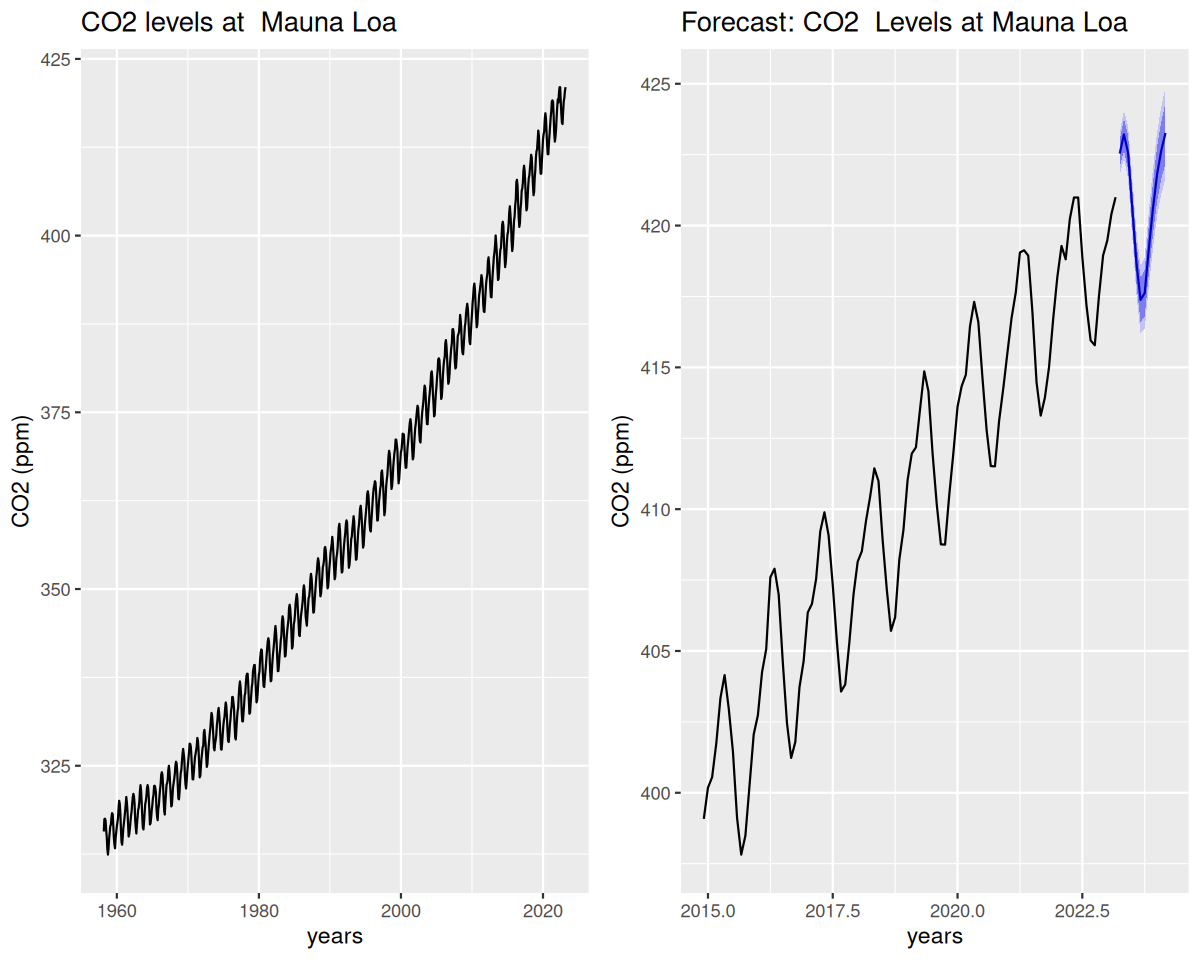
\includegraphics[width=0.75\linewidth]{figures/fig1-static-1} 

}

\caption{Left panel: CO2 Levels at Mauna Loa, time-series plot. The cardox data show a positive tendency and strong seasonality. Right panel: forecast of the next 12 months for the CO2 levels at Mauna Loa, the model's predictions capture the time-series behaviour.}\label{fig:fig1-static}
\end{figure}



\begin{verbatim}
library(forecast)
library(astsa)
model = ets(cardox)
summary(model)
#> ETS(M,A,A) 
#> 
#> Call:
#>  ets(y = cardox) 
#> 
#>   Smoothing parameters:
#>     alpha = 0.5451 
#>     beta  = 0.0073 
#>     gamma = 0.1076 
#> 
#>   Initial states:
#>     l = 314.4546 
#>     b = 0.0801 
#>     s = 0.6986 0.0648 -0.8273 -1.8999 -3.0527 -2.7629
#>            -1.2769 0.7015 2.1824 2.6754 2.3317 1.165
#> 
#>   sigma:  9e-04
#> 
#>      AIC     AICc      BIC 
#> 3429.637 3430.439 3508.867 
#> 
#> Training set error measures:
#>                    ME      RMSE       MAE         MPE       MAPE     MASE
#> Training set 0.018748 0.3158258 0.2476335 0.005051657 0.06933903 0.152935
#>                    ACF1
#> Training set 0.09308391
\end{verbatim}

The resulting model, proposed by the \texttt{ets()} function, for analyzing the \emph{carbon dioxide} data in \emph{Mauna Loa} is an \(ETS[M,A,A]\) model. The parameters \(\alpha, \beta \text{ and } \gamma\) (see Definition 1) have being estimated using the least squares method. If the assumptions on the model are satisfied, then the errors of the model behave like a Gaussian stationary process. To check it, we make use of the function \texttt{check\_residuals()}. For more details on the compatibility of this function with the models obtained by other packages see the \CRANpkg{nortsTest} repository. In the following, we display the results of using the \emph{Augmented Dickey-Fuller} test (\emph{Subsection 3.1}) to check the stationary assumption and the \emph{random projection} test with \texttt{k\ =\ 1} projections to check the normality assumption. For the other test options see the function's documentation.

\begin{verbatim}
check_residuals(model,unit_root = "adf",normality = "rp",
                   plot = TRUE)
\end{verbatim}

\begin{verbatim}
#> 
#>  *************************************************** 
#> 
#>  Unit root test for stationarity: 
#> 
#>  Augmented Dickey-Fuller Test
#> 
#> data:  y
#> Dickey-Fuller = -9.8935, Lag order = 9, p-value = 0.01
#> alternative hypothesis: stationary
#> 
#> 
#>  Conclusion: y is stationary
#>  *************************************************** 
#> 
#>  Goodness of fit test for Gaussian Distribution: 
#> 
#>  k random projections test.
#> 
#> data:  y
#> k = 1, p.value adjust = Benjamini & Yekutieli, p-value = 1
#> alternative hypothesis: y does not follow a Gaussian Process
#> 
#> 
#>  Conclusion: y follows a Gaussian Process
#>  
#>  ***************************************************
\end{verbatim}

The obtained results indicate that the null hypothesis of non stationarity is rejected at significance level \(\alpha = 0.01.\) Additionally, there is no evidence to reject the null hypothesis of normality at significance level \(\alpha = 0.05.\) Consequently, we conclude that the residuals follow a stationary Gaussian process, having that the resulting \(ETS[M,A,A]\) model adjusts well to the \emph{carbon dioxide} data in \emph{Mauna Loa}.

In the above displayed \texttt{check\_residuals()} function, the \texttt{plot} argument is set to \texttt{TRUE}. The resulting plots are shown in Figure \ref{fig:fig2-static}. The plot in the \emph{top} panel and the auto-correlation plots in the bottom panels insinuate that the residuals have a stationary behavior. The \emph{top} panel plot shows slight oscillations around zero and the auto-correlations functions in the \emph{bottom} panels have values close to zero in every lag. The histogram and qq-plot in the \emph{middle} panels suggest that the marginal distribution of the residuals is normally distributed. Therefore, Figure \ref{fig:fig2-static} agrees with the reported results, indicating that the assumptions of the model are satisfied.

\begin{figure}

{\centering 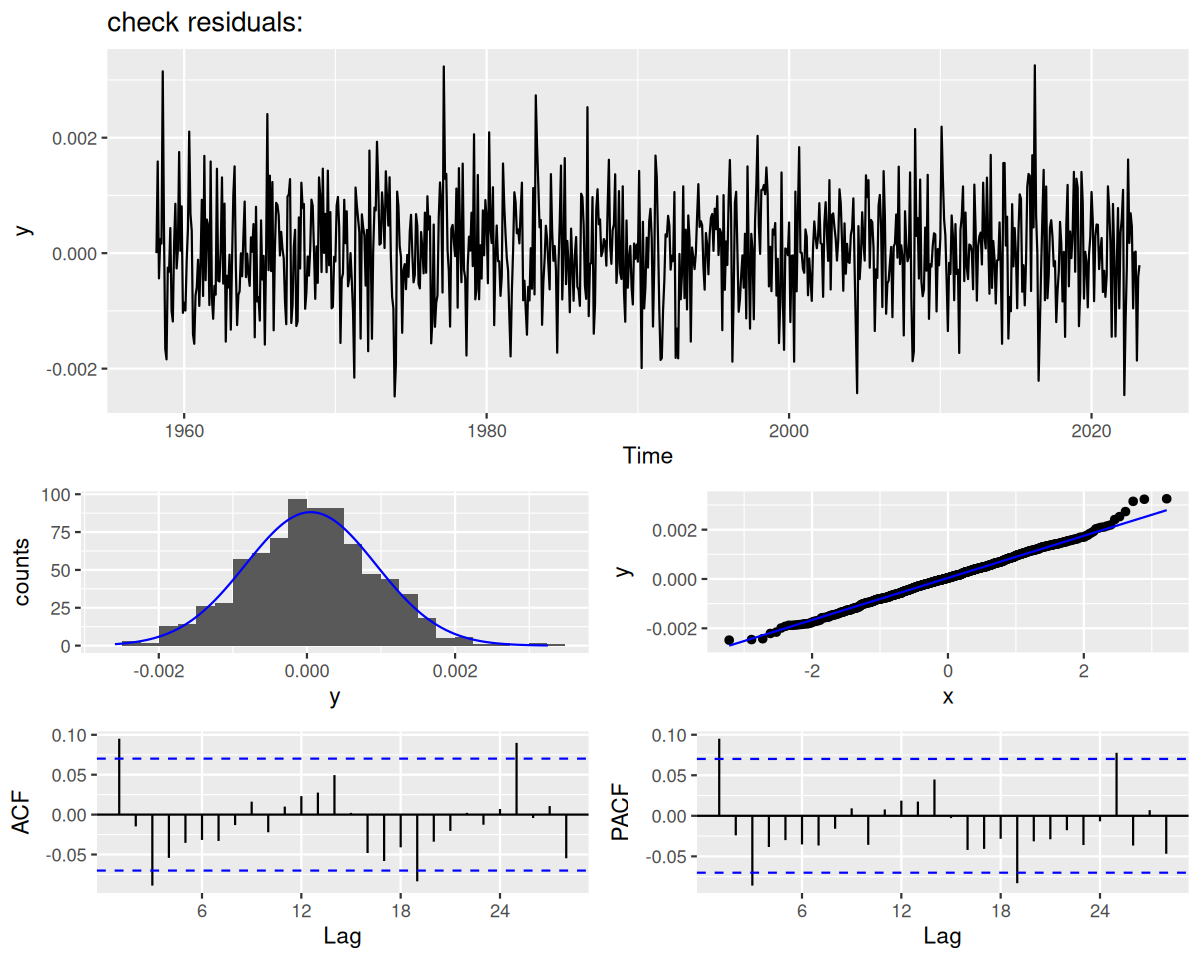
\includegraphics[width=1\linewidth]{figures/fig2-static-1} 

}

\caption{Check residuals plot for the ETS(M,A,A) model. The upper panel shows the residuals time-series plot, showing small oscillations around zero, which insinuates stationarity. The middle plots are the residuals histogram (middle-left) and quantile-quantile plot (middle-right), both plots suggest that the residuals have a normal distribution. The lower panel shows the autocorrelation functions, for both plots, the autocorrelations are close to zero giving the impression of stationarity.}\label{fig:fig2-static}
\end{figure}



As the assumptions of the model have been checked, it can be used for instance to forecast. The result of applying the following function is displayed in Figure \ref{fig:fig1-static}. It presents the carbon dioxide data for the last 8 years and a forecast of the next 12 months. It is observable from the plot that the model captures the process trend and periodicity.

\begin{verbatim}
autoplot(forecast(model,h = 12),include = 100,
         xlab = "years",ylab = "CO2 (ppm)",
         main = "Forecast: Carbon Dioxide Levels at Mauna Loa")
\end{verbatim}



\hypertarget{conclusions}{%
\section{Conclusions}\label{conclusions}}

For independent data, the \CRANpkg{nortest} package (Gross and Ligges 2015) provides five different tests for normality, the \CRANpkg{mvnormtest} package (Jarek 2012) performs the Shapiro-Wilks test for multivariate data and the \CRANpkg{MissMech} package (Jamshidian, Jalal, and Jansen 2014) provides tests for normality in multivariate incomplete data. To test the normality of dependent data, some authors such as Psaradakis and Vávra (2017) and Nieto-Reyes, Cuesta-Albertos, and Gamboa (2014) have available undocumented \texttt{Matlab} code, which is almost only helpful in re-doing their simulation studies.

To our knowledge, no consistent implementation or package of tests for normality of stationary processes has been done before. Therefore, the \CRANpkg{nortsTest} is the first package to implement normality tests in stationary processes. This work gives a general overview of a careful selection of tests for normality in the stationary process, which consists of the most available types of tests. It additionally provides examples that illustrate each of the test implementations.

For checking the model's assumptions, the \CRANpkg{forecast} and \CRANpkg{astsa} packages contain functions for visual diagnostic. Following the same idea, \CRANpkg{nortsTest} provides similar diagnostic methods; it also reports the results of testing stationarity and normality, the main assumptions for the residuals in time series analysis.

\hypertarget{future-work-and-projects}{%
\section{Future work and projects}\label{future-work-and-projects}}

A further version of the \CRANpkg{nortsTest} package will incorporate additional tests such as Bispectral (Hinich 1982) and Stein's characterization (Bontemps and Meddahi 2005). Further future work will include a Bayesian version of a \emph{residuals check} procedure that uses the random projection method. Any future version under development can be installed from \texttt{GitHub} using the following code.

\begin{verbatim}
if (!requireNamespace("remotes")) install.packages("remotes")
remotes::install_github("asael697/nortsTest",dependencies = TRUE)
\end{verbatim}

\hypertarget{acknowledgment}{%
\section*{Acknowledgment}\label{acknowledgment}}
\addcontentsline{toc}{section}{Acknowledgment}

This work was supported by grant PID2022-139237NB-I00 funded by ``ERDF A way of making Europe'' and MCIN/AEI/10.13039/501100011033.

\hypertarget{references}{%
\section*{References}\label{references}}
\addcontentsline{toc}{section}{References}

\hypertarget{refs}{}
\begin{CSLReferences}{1}{0}
\leavevmode\vadjust pre{\hypertarget{ref-vonMisses1962}{}}%
Anderson, T. W. 1962. {``{On the distribution of the two-sample Cramer-von Mises criterion}.''} \emph{The Annals of Mathematical Statistics} 33 (3): 1148--59. \url{https://doi.org/10.1214/aoms/1177704477}.

\leavevmode\vadjust pre{\hypertarget{ref-anderson1952}{}}%
Anderson, T. W., and D. A. Darling. 1952. {``Asymptotic Theory of Certain Goodness of Fit Criteria Based on Stochastic Processes.''} \emph{Annals of Mathematical Statistics} 23 (2): 193--212. \url{https://doi.org/10.1214/aoms/1177729437}.

\leavevmode\vadjust pre{\hypertarget{ref-bai2005}{}}%
Bai, Jushan, and Serena Ng. 2005. {``Tests for Skewness, Kurtosis, and Normality for Time Series Data.''} \emph{Journal of Business \& Economic Statistics} 23 (1): 49--60. \url{https://doi.org/10.1198/073500104000000271}.

\leavevmode\vadjust pre{\hypertarget{ref-Hegy1993}{}}%
Beaulieu, Joseph, and Jeffrey A. Miron. 1993. {``Seasonal Unit Roots in Aggregate {U.S.} Data.''} \emph{Journal of Econometrics} 55 (1): 305--28. \url{https://doi.org/10.1016/0304-4076(93)90018-Z}.

\leavevmode\vadjust pre{\hypertarget{ref-Benjamin1995}{}}%
Benjamini, Yoav, and Yosef Hochberg. 1995. {``Controlling the False Discovery Rate: A Practical and Powerful Approach to Multiple Testing.''} \emph{Journal of the Royal Statistical Society. Series B (Methodological)} 57 (1): 289--300. \url{http://www.jstor.org/stable/2346101}.

\leavevmode\vadjust pre{\hypertarget{ref-Benjamin2001}{}}%
Benjamini, Yoav, and Daniel Yekutieli. 2001. {``The Control of the False Discovery Rate in Multiple Testing Under Dependency.''} \emph{The Annals of Statistics} 29 (4): 1165--88. \url{http://www.jstor.org/stable/2674075}.

\leavevmode\vadjust pre{\hypertarget{ref-Berg2010}{}}%
Berg, Arthur, Efstathios Paparoditis, and Dimitris N. Politis. 2010. {``A Bootstrap Test for Time Series Linearity.''} \emph{Journal of Statistical Planning and Inference} 140 (12): 3841--57. \url{https://doi.org/10.1016/j.jspi.2010.04.047}.

\leavevmode\vadjust pre{\hypertarget{ref-Bollerslev1986}{}}%
Bollerslev, Tim. 1986. {``Generalized Autoregressive Conditional Heteroskedasticity.''} \emph{Journal of Econometrics} 31 (3): 307--27. \url{https://doi.org/10.1016/0304-4076(86)90063-1}.

\leavevmode\vadjust pre{\hypertarget{ref-Meddahi2005}{}}%
Bontemps, Christian, and Nour Meddahi. 2005. {``Testing Normality: A GMM Approach.''} \emph{Journal of Econometrics} 124 (1): 149--86. \url{https://doi.org/10.1016/j.jeconom.2004.02.014}.

\leavevmode\vadjust pre{\hypertarget{ref-Box}{}}%
Box, G. E. P., and David A. Pierce. 1970. {``Distribution of Residual Autocorrelations in Autoregressive-Integrated Moving Average Time Series Models.''} \emph{Journal of the American Statistical Association} 65 (332): 1509--26. \url{https://doi.org/10.1080/01621459.1970.10481180}.

\leavevmode\vadjust pre{\hypertarget{ref-Box1990}{}}%
Box, George Edward Pelham, and Gwilym Jenkins. 1990. \emph{Time Series Analysis, Forecasting and Control}. USA: Holden-Day, Inc. \url{https://www.wiley.com/en-us/Time+Series+Analysis}.

\leavevmode\vadjust pre{\hypertarget{ref-Buhlmann1997}{}}%
Bühlmann, Peter. 1997. {``Sieve Bootstrap for Time Series.''} \emph{Bernoulli} 3 (2): 123--48. \url{http://www.jstor.org/stable/3318584}.

\leavevmode\vadjust pre{\hypertarget{ref-ch1995}{}}%
Canova, Fabio, and Bruce E. Hansen. 1995. {``Are Seasonal Patterns Constant over Time? A Test for Seasonal Stability.''} \emph{Journal of Business \& Economic Statistics} 13 (3): 237--52. \url{https://doi.org/10.1080/07350015.1995.10524598}.

\leavevmode\vadjust pre{\hypertarget{ref-BIC2006}{}}%
Chen, Jiahua, and Zehua Chen. 2008. {``Extended Bayesian Information Criteria for Model Selection with Large Model Spaces.''} \emph{Biometrika} 95 (3): 759--71. \url{https://doi.org/10.1093/biomet/asn034}.

\leavevmode\vadjust pre{\hypertarget{ref-Cuesta2007}{}}%
Cuesta-Albertos, J. A., E. del Barrio, R. Fraiman, and C. Matrán. 2007. {``The Random Projection Method in Goodness of Fit for Functional Data.''} \emph{Computational Statistics \& Data Analysis} 51 (10): 4814--31. \url{https://doi.org/10.1016/j.csda.2006.09.007}.

\leavevmode\vadjust pre{\hypertarget{ref-Dagostino1987}{}}%
D'Agostino, Ralph B., and Michael A. Stephens. 1986. {``Goodness-of-Fit Techniques.''} \emph{Quality and Reliability Engineering International} 3 (1): 71--71. \url{https://doi.org/10.1002/qre.4680030121}.

\leavevmode\vadjust pre{\hypertarget{ref-Wilkinson1986}{}}%
Dallal, Gerard E., and Leland Wilkinson. 1986. {``An Analytic Approximation to the Distribution of Lilliefors's Test Statistic for Normality.''} \emph{The American Statistician} 40 (4): 294--96. \url{https://doi.org/10.1080/00031305.1986.10475419}.

\leavevmode\vadjust pre{\hypertarget{ref-DH2008}{}}%
Doornik, Jurgen A., and Henrik Hansen. 2008. {``{An omnibus test for univariate and multivariate normality}.''} \emph{Oxford Bulletin of Economics and Statistics} 70 (s1): 927--39. \url{https://doi.org/10.1111/j.1468-0084.2008.}

\leavevmode\vadjust pre{\hypertarget{ref-el2022normality}{}}%
El Bouch, Sara, Olivier Michel, and Pierre Comon. 2022. {``A Normality Test for Multivariate Dependent Samples.''} \emph{Signal Processing} 201: 108705. \url{https://doi.org/10.1016/j.sigpro.2022.108705}.

\leavevmode\vadjust pre{\hypertarget{ref-engle1982}{}}%
Engle, Robert F. 1982. {``Autoregressive Conditional Heteroscedasticity with Estimates of the Variance of United Kingdom Inflation.''} \emph{Econometrica} 50 (4): 987--1007. \url{http://www.jstor.org/stable/1912773}.

\leavevmode\vadjust pre{\hypertarget{ref-epps1987}{}}%
Epps, T. W. 1987. {``Testing That a Stationary Time Series Is {G}aussian.''} \emph{The Annals of Statistics} 15 (4): 1683--98. \url{https://doi.org/10.1214/aos/1176350618}.

\leavevmode\vadjust pre{\hypertarget{ref-Gasser1975}{}}%
Gasser, Theo. 1975. {``Goodness-of-Fit Tests for Correlated Data.''} \emph{Biometrika} 62 (3): 563--70. \url{http://www.jstor.org/stable/2335511}.

\leavevmode\vadjust pre{\hypertarget{ref-gelman2013}{}}%
Gelman, A., J. B. Carlin, H. S. Stern, D. B. Dunson, A. Vehtari, and D. B. Rubin. 2013. \emph{Bayesian Data Analysis, Third Edition}. Chapman \& Hall/CRC Texts in Statistical Science. Taylor \& Francis. \url{https://books.google.nl/books?id=ZXL6AQAAQBAJ}.

\leavevmode\vadjust pre{\hypertarget{ref-nortest2015}{}}%
Gross, Juergen, and Uwe Ligges. 2015. \emph{`Nortest`: Tests for Normality}. \url{https://CRAN.R-project.org/package=nortest}.

\leavevmode\vadjust pre{\hypertarget{ref-HZ1990}{}}%
Henze, N., and B. Zirkler. 1990. {``A Class of Invariant Consistent Tests for Multivariate Normality.''} \emph{Communications in Statistics - Theory and Methods} 19 (10): 3595--3617. \url{https://doi.org/10.1080/03610929008830400}.

\leavevmode\vadjust pre{\hypertarget{ref-Hinich1982}{}}%
Hinich, Melvin J. 1982. {``Testing for {G}aussianity and Linearity of a Stationary Time Series.''} \emph{Journal of Time Series Analysis} 3 (3): 169--76. \url{https://doi.org/10.1111/j.1467-9892.1982.tb00339}.

\leavevmode\vadjust pre{\hypertarget{ref-Holt2004}{}}%
Holt, Charles C. 2004. {``Forecasting Seasonals and Trends by Exponentially Weighted Moving Averages.''} \emph{International Journal of Forecasting} 20 (1): 5--10. \url{https://doi.org/10.1016/j.ijforecast.2003.09.015}.

\leavevmode\vadjust pre{\hypertarget{ref-hong1999hypothesis}{}}%
Hong, Yongmiao. 1999. {``Hypothesis Testing in Time Series via the Empirical Characteristic Function: A Generalized Spectral Density Approach.''} \emph{Journal of the American Statistical Association} 94 (448): 1201--20. \url{https://doi.org/10.2307/2669935}.

\leavevmode\vadjust pre{\hypertarget{ref-Hyndman2008}{}}%
Hyndman, Robin John, Anne B Koehler, J Keith Ord, and Ralph David Snyder. 2008. \emph{Forecasting with Exponential Smoothing: The State Space Approach}. Springer. \url{https://doi.org/10.1111/j.1751-5823.2009.00085_17}.

\leavevmode\vadjust pre{\hypertarget{ref-Rob2007}{}}%
Hyndman, Rob, and Yeasmin Khandakar. 2008. {``Automatic Time Series Forecasting: The `Forecast` Package for {`R`}.''} \emph{Journal of Statistical Software, Articles} 27 (3): 1--22. \url{https://doi.org/10.18637/jss.v027.i03}.

\leavevmode\vadjust pre{\hypertarget{ref-Mortaza2014}{}}%
Jamshidian, Mortaza, Siavash Jalal, and Camden Jansen. 2014. {```MissMech`: An {`R`} Package for Testing Homoscedasticity, Multivariate Normality, and Missing Completely at Random (MCAR).''} \emph{Journal of Statistical Software} 56 (6): 1--31. \url{http://www.jstatsoft.org/v56/i06/}.

\leavevmode\vadjust pre{\hypertarget{ref-mvnormtest2012}{}}%
Jarek, Slawomir. 2012. \emph{`Mvnormtest`: Normality Test for Multivariate Variables}. \url{https://CRAN.R-project.org/package=mvnormtest}.

\leavevmode\vadjust pre{\hypertarget{ref-jarque1980}{}}%
Jarque, Carlos M., and Anil K. Bera. 1980. {``Efficient Tests for Normality, Homoscedasticity and Serial Independence of Regression Residuals.''} \emph{Economics Letters} 6 (3): 255--59. \url{https://doi.org/10.1016/0165-1765(80)90024-5}.

\leavevmode\vadjust pre{\hypertarget{ref-KppsI1992}{}}%
Kwiatkowski, Denis, Peter C. B. Phillips, Peter Schmidt, and Yongcheol Shin. 1992. {``Testing the Null Hypothesis of Stationarity Against the Alternative of a Unit Root: How Sure Are We That Economic Time Series Have a Unit Root?''} \emph{Journal of Econometrics} 54 (1): 159--78. \url{https://doi.org/10.1016/0304-4076(92)90104-Y}.

\leavevmode\vadjust pre{\hypertarget{ref-Lobato2004}{}}%
Lobato, Ignacio, and Carlos Velasco. 2004. {``A Simple Test of Normality for Time Series.''} \emph{Econometric Theory} 20 (August): 671--89. \url{https://doi.org/10.1017/S0266466604204030}.

\leavevmode\vadjust pre{\hypertarget{ref-Lomincki1961}{}}%
Lomnicki, Z. 1961. {``Tests for Departure from Normality in the Case of Linear Stochastic Processes.''} \emph{Metrika: International Journal for Theoretical and Applied Statistics} 4 (1): 37--62. \url{https://EconPapers.repec.org/RePEc:spr:metrik:v:4:y:1961:i:1:p:37-62}.

\leavevmode\vadjust pre{\hypertarget{ref-uroot}{}}%
López-de-Lacalle, Javier. 2019. \emph{`Uroot`: Unit Root Tests for Seasonal Time Series}. \url{https://CRAN.R-project.org/package=uroot}.

\leavevmode\vadjust pre{\hypertarget{ref-mardia1970measures}{}}%
Mardia, Kanti V. 1970. {``Measures of Multivariate Skewness and Kurtosis with Applications.''} \emph{Biometrika} 57 (3): 519--30. \url{http://www.jstor.org/stable/2334770}.

\leavevmode\vadjust pre{\hypertarget{ref-meintanis2016review}{}}%
Meintanis, Simos G. 2016. {``A Review of Testing Procedures Based on the Empirical Characteristic Function.''} \emph{South African Statistical Journal} 50 (1): 1--14. \url{https://doi.org/10.10520/EJC186846}.

\leavevmode\vadjust pre{\hypertarget{ref-moulines1992testing}{}}%
Moulines, E, K Choukri, and M Sharbit. 1992. {``Testing That a Multivariate Stationary Time-Series Is {G}aussian.''} In \emph{{[}1992{]} IEEE Sixth SP Workshop on Statistical Signal and Array Processing}, 185--88. IEEE. \url{https://doi.org/10.1109/SSAP.1992.246818}.

\leavevmode\vadjust pre{\hypertarget{ref-Nieto-Reyes:2022-1}{}}%
Nieto-Reyes, Alicia. 2021. {``On the Non-{G}aussianity of the Height of Sea Waves.''} \emph{Journal of Marine Science and Engineering} 9 (12). \url{https://www.mdpi.com/2077-1312/9/12/1446}.

\leavevmode\vadjust pre{\hypertarget{ref-Nieto-Reyes:2022-2}{}}%
---------. 2022. {``On the Non-{G}aussianity of Sea Surface Elevations.''} \emph{Journal of Marine Science and Engineering} 10 (9). \url{https://doi.org/10.3390/jmse10091303}.

\leavevmode\vadjust pre{\hypertarget{ref-nietoreyes2014}{}}%
Nieto-Reyes, Alicia, Juan Antonio Cuesta-Albertos, and Fabrice Gamboa. 2014. {``A Random-Projection Based Test of {G}aussianity for Stationary Processes.''} \emph{Computational Statistics \& Data Analysis} 75: 124--41. \url{https://doi.org/10.1016/j.csda.2014.01.013}.

\leavevmode\vadjust pre{\hypertarget{ref-ocsb1988}{}}%
Osborn, Denise R., A. P. L. Chui, Jeremy P. Smith, and C. R. Birchenhall. 1988. {``Seasonality and the Order of Integration for Consumption.''} \emph{Oxford Bulletin of Economics and Statistics} 50 (4): 361--77. \url{https://doi.org/10.1111/j.1468-0084.1988.mp50004002.x}.

\leavevmode\vadjust pre{\hypertarget{ref-Pearson1895}{}}%
Pearson, Karl, and Olaus Magnus Friedrich Erdmann Henrici. 1895. {``X. {C}ontributions to the Mathematical Theory of Evolution.-{II} {S}kew Variation in Homogeneous Material.''} \emph{Philosophical Transactions of the Royal Society of London. (A.)} 186: 343--414. \url{https://doi.org/10.1098/rsta.1895.0010}.

\leavevmode\vadjust pre{\hypertarget{ref-Perron1988}{}}%
Perron, Pierre. 1988. {``Trends and Random Walks in Macroeconomic Time Series: Further Evidence from a New Spproach.''} \emph{Journal of Economic Dynamics and Control} 12 (2): 297--332. \url{https://doi.org/10.1016/0165-1889(88)90043-7}.

\leavevmode\vadjust pre{\hypertarget{ref-OBrien2010}{}}%
Petris, Giovanni, Sonia Petrone, and Patrizia Campagnoli. 2007. {``Dynamic Linear Models with {`R`}.''} Berlin: Springer. \url{https://doi.org/10.1111/j.1751-5823.2010.00109_26.x}.

\leavevmode\vadjust pre{\hypertarget{ref-MarianZach2017}{}}%
Psaradakis, Zacharias. 2017. {``Normality Tests for Dependent Data.''} Working and Discussion Papers WP 12/2017. Research Department, National Bank of Slovakia. \url{https://ideas.repec.org/p/svk/wpaper/1053.html}.

\leavevmode\vadjust pre{\hypertarget{ref-vavra2017}{}}%
Psaradakis, Zacharias, and Marián Vávra. 2017. {``A Distance Test of Normality for a Wide Class of Stationary Processes.''} \emph{Econometrics and Statistics} 2: 50--60. \url{https://doi.org/10.1016/j.ecosta.2016.11.005}.

\leavevmode\vadjust pre{\hypertarget{ref-psaradakis2020normality}{}}%
---------. 2020. {``Normality Tests for Dependent Data: Large-Sample and Bootstrap Approaches.''} \emph{Communications in Statistics-Simulation and Computation} 49 (2): 283--304. \url{https://doi.org/10.1080/03610918.2018.1485941}.

\leavevmode\vadjust pre{\hypertarget{ref-mvntest}{}}%
Pya, Natalya, Vassilly Voinov, Rashid Makarov, and Yevgeniy Voinov. 2016. \emph{`mvnTest`: Goodness of Fit Tests for Multivariate Normality}. \url{https://CRAN.R-project.org/package=mvnTest}.

\leavevmode\vadjust pre{\hypertarget{ref-aTSA}{}}%
Qiu, Debin. 2015. \emph{`aTSA`: Alternative Time Series Analysis}. \url{https://CRAN.R-project.org/package=aTSA}.

\leavevmode\vadjust pre{\hypertarget{ref-Royston1982}{}}%
Royston, J. P. 1982. {``An Extension of {S}hapiro and {W}ilk's {W} Test for Normality to Large Samples.''} \emph{Journal of the Royal Statistical Society. Series C (Applied Statistics)} 31 (2): 115--24. \url{http://www.jstor.org/stable/2347973}.

\leavevmode\vadjust pre{\hypertarget{ref-Royston1992}{}}%
---------. 1992. {``Approximating the Shapiro-Wilk {W}-Test for Non-Normality.''} \emph{Journal of Statistics and Computing} 2 (3): 117--19. \url{https://doi.org/10.1007/BF01891203}.

\leavevmode\vadjust pre{\hypertarget{ref-Royston1993}{}}%
Royston, Patrick. 1993. {``A Pocket-Calculator Algorithm for the {S}hapiro-{F}rancia Test for Non-Normality: An Application to Medicine.''} \emph{Statistics in Medicine} 12 (2): 181--84. \url{https://doi.org/10.1002/sim.4780120209}.

\leavevmode\vadjust pre{\hypertarget{ref-dickey1984}{}}%
Said, Said E., and David A. Dickey. 1984. {``Testing for Unit Roots in Autoregressive-Moving Average Models of Unknown Order.''} \emph{Biometrika} 71 (3): 599--607. \url{https://doi.org/10.1093/biomet/71.3.599}.

\leavevmode\vadjust pre{\hypertarget{ref-SWtest1965}{}}%
Shapiro, S. S., and M. B. Wilk. 1965. {``An Analysis of Variance Test for Normality (Complete Samples).''} \emph{Biometrika} 52 (3-4): 591--611. \url{https://doi.org/10.1093/biomet/52.3-4.591}.

\leavevmode\vadjust pre{\hypertarget{ref-shumway2010}{}}%
Shumway, R. H., and D. S. Stoffer. 2010. \emph{Time Series Analysis and Itts Applications: With {`R`} Examples}. Springer Texts in Statistics. Springer New York. \url{https://books.google.es/books?id=dbS5IQ8P5gYC}.

\leavevmode\vadjust pre{\hypertarget{ref-Smirnov1948}{}}%
Smirnov, N. 1948. {``Table for Estimating the Goodness of Fit of Empirical Distributions.''} \emph{Annals of Mathematical Statistics} 19 (2): 279--81. \url{https://doi.org/10.1214/aoms/1177730256}.

\leavevmode\vadjust pre{\hypertarget{ref-Steinberg1992}{}}%
Steinberg, Y., and O. Zeitouni. 1992. {``On Tests for Normality.''} \emph{IEEE Transactions on Information Theory} 38 (6): 1779--87. \url{https://doi.org/10.1109/18.165450}.

\leavevmode\vadjust pre{\hypertarget{ref-astsa}{}}%
Stoffer, David. 2020. \emph{`Astsa`: Applied Statistical Time Series Analysis}. \url{https://CRAN.R-project.org/package=astsa}.

\leavevmode\vadjust pre{\hypertarget{ref-R}{}}%
Team, `R` Core. 2018. \emph{{`R`}: A Language and Environment for Statistical Computing}. Vienna, Austria: {`R`} Foundation for Statistical Computing. \url{https://www.R-project.org/}.

\leavevmode\vadjust pre{\hypertarget{ref-tseries}{}}%
Trapletti, Adrian, and Kurt Hornik. 2019. \emph{`Tseries`: Time Series Analysis and Computational Finance}. \url{https://CRAN.R-project.org/package=tseries}.

\leavevmode\vadjust pre{\hypertarget{ref-Ts2010}{}}%
Tsay, R. 2010. \emph{Analysis of Financial Time Series}. Second. Chicago: Wiley-Interscience. \url{https://doi.org/10.1002/0471264105}.

\leavevmode\vadjust pre{\hypertarget{ref-S2_2016}{}}%
Vassilly Voinov, Rashid Makarov, Natalie Pya, and Yevgeniy Voinov. 2016. {``New Invariant and Consistent Chi-Squared Type Goodness-of-Fit Tests for Multivariate Normality and a Related Comparative Simulation Study.''} \emph{Communications in Statistics - Theory and Methods} 45 (11): 3249--63. \url{https://doi.org/10.1080/03610926.2014.901370}.

\leavevmode\vadjust pre{\hypertarget{ref-W2006}{}}%
Wasserman, Larry. 2006. \emph{All of Nonparametric Statistics}. New York: Springer. \url{https://doi.org/10.1007/0-387-30623-4}.

\leavevmode\vadjust pre{\hypertarget{ref-west2006}{}}%
West, M., and J. Harrison. 2006. \emph{Bayesian Forecasting and Dynamic Models}. Springer Series in Statistics. Springer New York. \url{https://books.google.nl/books?id=0mPgBwAAQBAJ}.

\leavevmode\vadjust pre{\hypertarget{ref-ggplot2}{}}%
Wickham, Hadley. 2009. \emph{`Ggplot2`: Elegant Graphics for Data Analysis}. Springer-Verlag New York. \url{http://ggplot2.org}.

\leavevmode\vadjust pre{\hypertarget{ref-cowplot}{}}%
Wilke, Claus O. 2020. \emph{`Cowplot`: Streamlined Plot Theme and Plot Annotations for `Ggplot2`}. \url{https://CRAN.R-project.org/package=cowplot}.

\leavevmode\vadjust pre{\hypertarget{ref-fGarch}{}}%
Wuertz, Diethelm, Tobias Setz, Yohan Chalabi, Chris Boudt, Pierre Chausse, and Michal Miklovac. 2017. \emph{`fGarch`: Rmetrics - Autoregressive Conditional Heteroskedastic Modelling}. \url{https://CRAN.R-project.org/package=fGarch}.

\end{CSLReferences}

\bibliography{RJreferences.bib}

\address{%
Asael Alonzo Matamoros\\
Aalto University\\%
Department of Computer Science\\ Eespo, Finland\\
%
\url{https://asael697.github.io}\\%
%
\href{mailto:izhar.alonzomatamoros@aalto.fi}{\nolinkurl{izhar.alonzomatamoros@aalto.fi}}%
}

\address{%
Alicia Nieto-Reyes\\
Universidad de Cantabria\\%
Departmento de Mathemáticas, Estadística y Computación\\ Avd. de los Castros s/n.~39005 Santander, Spain\\
%
\url{https://orcid.org/0000-0002-0268-3322}\\%
%
\href{mailto:alicia.nieto@unican.es}{\nolinkurl{alicia.nieto@unican.es}}%
}

\address{%
Claudio Agostinelli\\
University of Trento\\%
Department of Mathematics\\ Via Sommarive, 14 - 38123 Povo\\
%
\url{https://orcid.org/0000-0001-6702-4312}\\%
%
\href{mailto:claudio.agostinelli@unitn.it}{\nolinkurl{claudio.agostinelli@unitn.it}}%
}
